\documentclass[11pt]{article}

\usepackage{amsthm}
\usepackage{amssymb}
\usepackage{amsmath}
\usepackage{cite}
\usepackage{hyperref}
\usepackage{mathtools}
\usepackage{subcaption}
\usepackage{tikz}
\usepackage{float}
\usepackage{caption}
\usepackage[nottoc]{tocbibind}
\usepackage[english]{babel}
\usepackage[utf8x]{inputenc}
\usepackage{venndiagram}
\usepackage{xspace}
\usepackage{centernot}
\usepackage[linesnumbered,ruled,lined,boxed,vlined,noend]{algorithm2e}
\usepackage[[deletedmarkup=xout, commentmarkup=footnote]{changes}
\usepackage{mathtools}

\newsavebox{\largestimage}

\newcommand{\accente}{\`E }

\newcommand{\splitfunc}{\textup{Split}}
\newcommand{\rankfunc}{\textup{rank}}
\newcommand{\rankfuncnomath}{\emph{rank}\xspace}
\newcommand{\rscp}{\textup{RSCP}}
\newcommand{\rscpnomath}{\emph{RSCP}\xspace}
\newcommand{\prefunc}{\textup{Pre}}
\newcommand{\prefuncnomath}{\emph{Pre}\xspace}
\newcommand{\succfunc}{\textup{Succ}}
\newcommand{\succfuncnomath}{\emph{Succ}\xspace}

\makeatletter
\renewcommand{\boxed}[1]{\text{\fboxsep=.2em\fbox{\m@th$\displaystyle#1$}}}
\makeatother

\newcommand\restr[2]{{% we make the whole thing an ordinary symbol
  \left.\kern-\nulldelimiterspace % automatically resize the bar with \right
  #1 % the function
  \vphantom{\big|} % pretend it's a little taller at normal size
  \right|_{#2} % this is the delimiter
  }}

\newcommand\sccto{\stackrel{\mathclap{\normalfont\mbox{\tiny{SCC}}}}{\to}}
\newcommand\superscc{\scalebox{.5}{SCC}}

\definechangesauthor[name=Alberto Casagrande, color=red]{ac}

\usetikzlibrary{arrows,automata,patterns,shapes,snakes,arrows.meta}

\graphicspath{ {imgs/} }

\captionsetup[figure]{name=Figura}
\captionsetup[table]{name=Tabella}
\renewcommand{\algorithmcfname}{Algoritmo}
\renewcommand\labelitemi{--}

\SetArgSty{textnormal}

\theoremstyle{definition}
\newtheorem{definition}{Definizione}[section]
\newtheorem{example}{Esempio}[section]
\newtheorem{axiom}{Assioma}[section]
\newtheorem*{axiom*}{Assioma}
\newtheorem{observation}{Osservazione}[section]
\newtheorem*{observation*}{Osservazione}

\theoremstyle{plain}
\newtheorem{proposition}{Proposizione}[section]
\newtheorem{lemma}{Lemma}[section]
\newtheorem{theorem}{Teorema}[section]
\newtheorem{corollary}{Corollario}[section]

\newcommand{\notimplies}{\mathrel{{\ooalign{\hidewidth$\not\phantom{=}$\hidewidth\cr$\implies$}}}}

\newenvironment{proof2}
{
  \begin{proof}[Dimostrazione]
}
{\end{proof}}

\includeonly{sezione3/file}

\begin{document}

\renewcommand\contentsname{Indice}
\tableofcontents
\addtocontents{toc}{~\hfill\textbf{Pagina}\par}

\subsection{Relazioni Binarie}
Riportiamo la definizione di \emph{relazione binaria} su uno o due insiemi, che sarà utile per definire formalmente il concetto di \emph{grafo}, fondamentale all'interno di questo elaborato:
\begin{definition}
    Una \emph{relazione binaria} su $A,B$ è un sottoinsieme del prodotto cartesiano $A \times B$.\\
    Una \emph{relazione binaria} su $A$ è un sottoinsieme del prodotto cartesiano $A \times A$.\\
	Se $R$ mette in relazione $u,v$, cioè $(u,v) \in R$, si usa la notazione $u R v$.
\end{definition}
\begin{definition}
    L' \emph{insieme immagine} di un elemento $x$ dell'insieme $A$ attraverso la relazione $R$ è l'insieme $R(x) = \{y \in B \mid x R y\}$.
\end{definition}
Alcune relazioni binarie mostrano proprietà fondamentali, che presentiamo nella definizione seguente:
\begin{definition}
    Sia $R$ una relazione binaria su $A$. Siano $x,y,z$ qualsiasi appartenenti ad $A$. Allora $R$ è:
    \begin{itemize}
        \item \emph{Riflessiva} se $x R x$;
        \item \emph{Simmetrica} se $x R y \implies y R x$;
        \item \emph{Transitiva} se $(x R y \land y R z) \implies x R z$.
    \end{itemize}
\end{definition}
\begin{example}
    La relazione ``$\leq$'' sui naturali è riflessiva e transitiva, ma non simmetrica. La relazione ``$=$'' ($a = b \iff $``$a,b$ sono lo stesso numero'') sui naturali è simmetrica, riflessiva e transitiva.
\end{example}
\begin{definition}
    Una \emph{relazione di equivalenza} su un insieme $A$ è una relazione binaria riflessiva, simmetrica e transitiva. Si vede facilmente che questo genere di relazione partiziona $A$ in \emph{classi di equivalenza}, ovvero sottoinsiemi disgiunti di $A$ all'interno dei quali tutte le coppie di elementi sono in relazione.
\end{definition}
Data una relazione di equivalenza $R$ su un insieme $A$, si usa la notazione ``$[a]_R$'' per indicare la classe di equivalenza di $R$ a cui appartiene $a$. Inoltre si usa la notazione ``$A/R$'', che si legge ``\emph{quoziente} di $A$ rispetto a $R$'', per denotare l'insieme delle classi di equivalenza di $R$ su $A$.\\
In alcune situazioni risulta conveniente definire la più piccola relazione (cioè quella che mette in relazione il minor numero possibile di coppie) che dispone di una certa proprietà, e che contiene una relazione binaria di partenza. Una relazione costruita in questo modo è una ``\emph{chiusura}'':
\begin{definition}
	Sia $R$ una relazione binaria su $A$. Le seguenti relazioni sono chiusure di $R$:
    \begin{itemize}
        \item \emph{Riflessiva}: $R_r = R \cup \{(x,x) \mid x \in A\}$;
        \item \emph{Simmetrica}: $R_s = R \cup \{(y,x) \mid x R y\}$;
        \item \emph{Transitiva}: $R_t = R \cup \{(x,z) \mid \exists y \in A,\, x R y \land y R z\}$.
    \end{itemize}
\end{definition}
\begin{example}
    La chiusura riflessiva della relazione ``$<$'' (minore stretto) è la relazione ``$\leq$''.
\end{example}
Nel seguito useremo ampiamente la definizione seguente:
\begin{definition}
    Sia $R$ una relazione binaria su $A \times B$. La \emph{contro-immagine} di un elemento $y \in B$ rispetto ad $R$ è l'insieme $R^{-1}(y) = \{x \in A \mid x R y\}$.\\
    Più in generale, la \emph{funzione inversa} di $R$ è la funzione $R^{-1} : \mathcal{P}(B) \to \mathcal{P}(A)$ (dove ``$\mathcal{P}$'' denota l'insieme delle parti) che associa ad un sottoinsieme di $B$ tutti gli $x \in A$ tali che vale $x R y$ per almeno un $y$ del sottoinsieme.
\end{definition}
Adottiamo infine la notazione ``$|A|$'' per indicare la \emph{cardinalità} dell'insieme $A$. In modo analogo, data una relazione binaria $R$, $|R|$ è il numero delle coppie messe in relazione da $R$.

\subsection{Grafi}
Il problema che intendiamo affrontare in questo elaborato è descritto con il formalismo della teoria dei grafi. In questa sezione presentiamo un sottoinsieme minimale di definizioni e risultati che ci consentirà di introdurre e trattare la questione.

\subsubsection{Definizione e generalità}
Con le premesse viste sopra possiamo definire un \emph{grafo} come segue:
\begin{definition}
    Sia $V$ un insieme finito non vuoto. Sia $E$ una relazione binaria su $V$. La coppia $G = (V, E)$ è un \emph{grafo diretto} (o \emph{orientato}). Con questa notazione:
    \begin{itemize}
        \item $V$ è l'insieme dei \emph{nodi} (o \emph{vertici});
        \item $E$ è una relazione binaria (in generale non simmetrica) che mette in relazione alcuni dei nodi di $G$.
    \end{itemize}
\end{definition}
\begin{example}
    \begin{figure}[t]
        \centering
        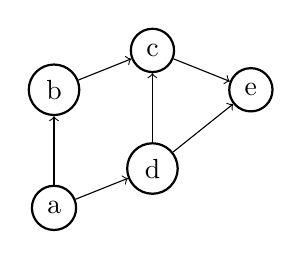
\begin{tikzpicture}[scale=0.5]
            \begin{scope}[every node/.style={circle,thick,draw}]
                \node (a) at (0,0) {a};
                \node (b) at (0,3) {b};
                \node (c) at (2.5,4) {c};
                \node (d) at (2.5,1) {d};
                \node (e) at (5,3) {e};
            \end{scope}

            \begin{scope}
                \path [->] (a) edge node {} (b);
                \path [->] (b) edge node {} (c);
                \path [->] (a) edge node {} (d);
                \path [->] (d) edge node {} (c);
                \path [->] (d) edge node {} (e);
                \path [->] (c) edge node {} (e);
            \end{scope}
            \end{tikzpicture}
        \caption{Rappresentazione grafica di un grafo diretto}
        \label{fig:graph}
    \end{figure}
    Il grafo di Figura \ref{fig:graph} è descritto dalla coppia
    \begin{itemize}
        \item $V = \{a,b,c,d,e\}$
        \item $E = \{(a,b), (a,d), (b,c), (d,c), (c,e), (d,e)\}$
    \end{itemize}
\end{example}
Nel seguito utilizzeremo ampiamente la seguente terminologia:
\begin{definition}
    Sia $G = (V,E)$ un grafo diretto. Consideriamo un arco $(u,v) \in E$. In questo caso $u$ è la \emph{sorgente} dell'arco, mentre $v$ è la \emph{destinazione}. Se il numero di archi uscenti da un nodo è zero, allora tale nodo  è un \emph{pozzo} (dall'inglese \emph{sink}).
\end{definition}

\subsubsection{Componenti fortemente connesse}
Come abbiamo visto sopra, un grafo diretto è un insieme di elementi (i \emph{nodi}) accoppiato con un insieme di relazioni tra questi elementi (gli \emph{archi}). \accente naturale associare questo concetto all'idea di percorso: ogni grafo è definito da un insieme di nodi ed un insieme di \emph{cammini} che consentono di spostarsi da un nodo ad un altro. La seguente definizione sorge in modo spontaneo da questa interpretazione:
\begin{definition}
    Sia $G = (V, E)$ un grafo diretto. Siano $u,v \in V$. $v$ \emph{è raggiungibile} da $u$, o in alternativa \emph{esiste un cammino} da $u$ a $v$, o ancora $u E^{*} v$, se esiste una sequenza finita di nodi $\displaystyle \{x_n\}_{n \in \{0,\dots,K\}}$, tale che $x_0 = u, x_K = v, x_n E x_{n+1}$.
\end{definition}
L'esistenza di un cammino tra nodi fornisce un criterio immediato per partizionare un grafo in gruppi di nodi. Diamo innanzitutto la seguente definizione:
\begin{definition}
    Un grafo diretto $(V,E)$ è \emph{fortemente connesso} se per ogni coppia di nodi $v_1, v_2 \in V$ esiste un cammino da $v_1$ a $v_2$, cioè $v_1 E^{*} v_2$.
\end{definition}
Allora possiamo individuare i sottografi massimali (cioè la ripartizione del grafo in sottografi che consente di minimizzare il numero di sottografi) fortemente connessi (\hspace*{-0.1cm}\cite[Appendice B]{clrs}):
\begin{definition}
    Le \emph{componenti fortemente connesse} (\emph{strongly connected components}, \emph{SCC}) di un grafo diretto sono i sottografi che compongono la ripartizione (massimale) del grafo in sottografi fortemente connessi.
\end{definition}
\begin{example}
    \begin{figure}[t]
        \centering
        \begin{tikzpicture}[scale=0.5]
            \begin{scope}[every node/.style={circle,thick,draw}]
                \node (a) at (0,0) {a};
                \node (b) at (0,3) {b};
                \node (c) at (2.5,4) {c};
                \node (d) at (2.5,1) {d};
                \node (e)[diamond] at (5,3) {e};
            \end{scope}

            \begin{scope}
                \path [->] (a) edge node {} (b);
                \path [->] (b) edge node {} (c);
                \path [->] (d) edge node {} (a);
                \path [->] (c) edge node {} (d);
                \path [->] (d) edge node {} (e);
                \path [->] (c) edge node {} (e);
            \end{scope}
            \end{tikzpicture}
        \caption{SCC di un grafo diretto}
        \label{fig:graph_cfc_1}
    \end{figure}
    Nel grafo di Figura \ref{fig:graph_cfc_1} le SCC sono rappresentate con forme diverse: $\{a,b,c,d\}, \{e\}$.
\end{example}
Il partizionamento dei nodi in SCC è definito come segue:
\begin{definition} \label{def:scc_partition}
    Sia $G = (V, E)$ un grafo diretto. Il grafo $G^{\superscc} = (V^{\superscc}, E^{\superscc})$, dove:
    \begin{itemize}
        \item $V^{\superscc} = \{C \mid \,C$ è una SCC$\}$;
        \item $E^{\superscc} = \{(A,B) \in V^{\superscc} \times V^{\superscc} \mid A \neq B, \exists m \in A, n \in B, m E n\}$
    \end{itemize}
    è il partizionamento del grafo iniziale in SCC.
\end{definition}
Riportiamo la seguente proprietà immediata:
\begin{proposition}
    Sia $G^{\superscc}$ il grafo delle SCC di un grafo $G$ generico. Allora $G^{\superscc}$ è aciclico.
\end{proposition}
\begin{proof2}
    Supponiamo per assurdo che in $G^{\superscc}$ esista un ciclo. Allora tutti i nodi di $V^{\superscc}$ facenti parte del ciclo sono mutuamente raggiungibili (percorrendo il ciclo). Quindi tutti i nodi fanno parte della stessa SCC, ma questo è assurdo.
\end{proof2}
\begin{example}
    \begin{figure}[t]
        \centering
        \begin{subfigure}{.45\textwidth}
          \centering
          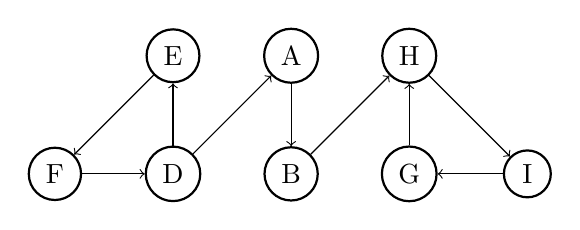
\begin{tikzpicture}[scale=0.5]
            \begin{scope}[every node/.style={circle,thick,draw}]
                \node (A) at (0,3) {A};
                \node (B) at (0,0) {B};

                \node (D) at (-3,0) {D};
                \node (E) at (-3,3) {E};
                \node (F) at (-6,0) {F};

                \node (G) at (3,0) {G};
                \node (H) at (3,3) {H};
                \node (I) at (6,0) {I};
            \end{scope}

            \begin{scope}
                \path [->] (A) edge node {} (B);

                \path [->] (E) edge node {} (F);
                \path [->] (F) edge node {} (D);
                \path [->] (D) edge node {} (E);

                \path [->] (G) edge node {} (H);
                \path [->] (H) edge node {} (I);
                \path [->] (I) edge node {} (G);

                \path [->] (D) edge node {} (A);
                \path [->] (B) edge node {} (H);
            \end{scope}
            \end{tikzpicture}
          \caption{Un grafo}
        \end{subfigure}
        \hfill
        \begin{subfigure}{.45\textwidth}
          \centering
          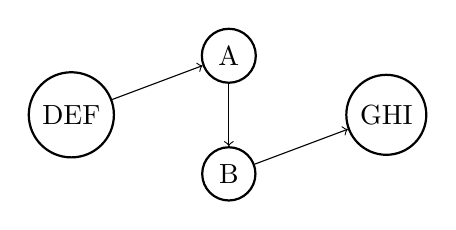
\begin{tikzpicture}[scale=0.5]
            \begin{scope}[every node/.style={circle,thick,draw}]
                \node (A) at (0,3) {A};
                \node (B) at (0,0) {B};

                \node (DEF) at (-4,1.5) {DEF};

                \node (GHI) at (4,1.5) {GHI};
            \end{scope}
                \path [->] (A) edge node {} (B);
                \path [->] (DEF) edge node {} (A);
                \path [->] (B) edge node {} (GHI);
            \begin{scope}

            \end{scope}
            \end{tikzpicture}
          \caption{Corrispondente grafo delle SCC}
        \end{subfigure}
        \caption{Un grafo ed il corrispondente grafo delle SCC}
        \label{fig:graph_cfc_2}
    \end{figure}
    La Figura \ref{fig:graph_cfc_2}.a rappresenta un grafo diretto generico, la Figura \ref{fig:graph_cfc_2}.b rappresenta il suo grafo delle componenti fortemente connesse associato.
\end{example}
Dato un grafo diretto generico possiamo determinare la ripartizione in SCC dei suoi nodi sfruttando un algoritmo avente complessità lineare $\Theta(|V| + |E|)$ \cite{tarjan}. L'algoritmo non verrà trattato in questo elaborato.\\

\subsubsection{Visita in profondità}
Delle due metodologie prevalenti per l'esplorazione di un grafo, \emph{visita in ampiezza} (\emph{Breadth-First-Search}, abbreviato in BFS) e \emph{visita in profondità} (\emph{Depth-First-Search}, abbreviato in DFS), in questo lavoro ci interessiamo alla seconda. Come dice il nome, questa tecnica consiste nella visita esaustiva di tutti i figli di un nodo, prima di passare agli altri nodi sullo stesso livello. Riportiamo lo pseudocodice da \cite{clrs}, leggermente modificato:\\
\begin{algorithm}[H]
    \label{alg:dfs}
    \KwData{$G = (V,E)$}
    \caption{DFS}
    \SetAlgoLined
    \SetKwProg{Fn}{function}{:}{end}
    \Fn{\textup{dsf-visit}($G = (V,E), n,$ time)}{
        n.color = GRAY\;
        \ForAll{$m \mid (nEm \land m.$color = WHITE)}{
            time = dfs-visit($G, m,$ time)\;
        }
        n.finishing-time = time\;
        n.color = BLACK\;
        time = time+1\;
        \Return{time}\;
    }
    \Begin{
        \ForAll{$n \in V$}{
            n.color = WHITE\;
        }

        time = 0\;
        \While{$\exists n \in V \mid n.color ==$ WHITE}{
            time = dfs-visit($G,n,$ time)\;
        }
    }
\end{algorithm}
L'attributo \emph{color} dei nodi del grafo consente di distinguere tra quei nodi che sono già stati visitati in modo esauriente (colore nero), quelli per cui è in corso una visita in profondità (colore grigio) e quelli non ancora esaminati dall'algoritmo (colore bianco). Si osservi che la colorazione dei nodi non è solamente accessoria, ma fornisce un meccanismo per evitare un loop infinito nel caso in cui il grafo contenga un ciclo.

Oltre alla colorazione dei nodi, l'algoritmo imposta l'attributo \emph{finishing-time} per ogni nodo, ovvero l'istante di tempo (a partire da \emph{time} $= 0$) in cui è stata terminata la visita esaustiva in profondità per tale nodo. Nello pseudocodice completo vengono considerati altri due attributi: \emph{starting-time} e \emph{parent}. Questi ultimi tre attributi forniscono alcune importanti proprietà all'algoritmo di visita in profondità, che non saranno approfondite in questo lavoro (si vedano \emph{Parenthesis theorem}, \emph{White-path theorem} in \cite{clrs}).

L'attributo \emph{finishing-time} è sufficiente per alcune applicazioni che saranno esposte nelle sezioni seguenti.

\subsection{Insiemi}
\subsubsection{Cenni di teoria degli insiemi}
In generale supporremo validi gli assiomi su cui si fonda la teoria degli insiemi ZFC, ad eccezione dell'Assioma di Fondazione. Diamo innanzitutto una formulazione degli assiomi che interverranno nel seguito del lavoro:
\begin{axiom}[di estensionalità]
    Due insiemi sono uguali $\iff$ contengono gli stessi elementi.
\end{axiom}
\begin{axiom}[di fondazione]
    Ogni insieme non vuoto contiene un elemento disgiunto dall'insieme stesso.
    \label{axi:foundation}
\end{axiom}
Del primo faremo un uso esplicito nel seguito. Il secondo, per motivi che saranno evidenti nella sezione seguente, risulta limitante nell'ambito trattato in questo elaborato. Introduciamo la seguente definizione:
\begin{definition}
    Un insieme è \emph{ben-fondato} se non contiene se stesso. Altrimenti è \emph{non-ben-fondato}.
\end{definition}
\begin{example}
    L'insieme $\Omega = \{\Omega\}$ è non-ben-fondato. L'insieme $A = \{1,2,3\}$ è ben-fondato.
\end{example}
Riportiamo una formulazione equivalente dell'Assioma \ref{axi:foundation}:
\begin{axiom*}[\ref{axi:foundation} bis]
    $\forall A$ la relazione ``$\in$'' è ben-fondata su $A$ \cite[Chapter III.4]{kunen}
\end{axiom*}
Da questa questa formulazione risulta evidente l'impossibilità, in ZFC, di costruire insiemi non-ben-fondati.

Rinunciando all'Assioma \ref{axi:foundation} si ottiene un sistema di assiomi che ammette l'esistenza di insiemi non-ben-fondati; tuttavia si può verificare che questo sistema non è più sufficiente a descrivere in modo esaustivo l'aritmetica per mezzo di operazioni su insiemi. Per ovviare a questa mancanza si introduce l'Assioma AFA, che verrà presentato e discusso nella sezione seguente.

% TODO: definisci insieme ereditariamente finito (si può costruire a partire dall'insieme vuoto utilizzando solamente il costruttore {} vedi ZFC) e insime non-ben-fondato prima di usare i grafi per rappresentare gli insiemi

\subsubsection{Rappresentazione di insiemi tramite grafi diretti}
\label{sec:graphs_sets}
In alcuni casi risulta conveniente fornire un'in\-ter\-pre\-ta\-zio\-ne insiemistica della nozione di grafo vista sopra. Introduciamo innanzitutto un concetto fondamentale per il seguito del lavoro:
\begin{definition}
    Sia $G = (V, E)$ un grafo diretto. Supponiamo che esista un $u \in V$ tale che ogni vertice del grafo è raggiungibile da $u$. Allora la coppia $(G, u)$ è un \emph{accessible pointed graph}, o \emph{APG}.
\end{definition}
Per rappresentare un insieme tramite un grafo diretto è necessario definire un processo denominato \emph{decorazione}:
\begin{definition}
    La \emph{decorazione} di un APG è l'assegnazione di un insieme ad ogni suo nodo. In tal caso viene associata la relazione ``$\in$'' alla relazione di raggiungibilità ``$E$'', ovvero $aEb \iff b \in a$.
\end{definition}
Possiamo ora dare la seguente definizione:
\begin{definition}
    L'\emph{immagine} (o \emph{picture} in \cite{aczel}) di un insieme $A$ è la coppia composta da un APG $(G,v)$ e da una sua decorazione in cui a $v$ è associato $A$.
\end{definition}
Vale la seguente proposizione, dimostrata in \cite{aczel}:
\begin{proposition}
    Ad un APG aciclico è possibile associare un'unica decorazione.
\end{proposition}
Questo risultato non è stato dimostrato nel caso di un APG contenente almeno un ciclo. Per questo motivo viene introdotto il seguente assioma:
\begin{axiom}[AFA, Anti-Foundation-Axiom]
    Ogni APG possiede un'unica decorazione.
\end{axiom}
L'assioma AFA ha un'ovvia conseguenza:
\begin{corollary}
    Ogni APG è immagine di un unico insieme.
\end{corollary}
\begin{example}
    \begin{figure}[b]
        \centering
        \begin{subfigure}{.25\textwidth}
          \centering
          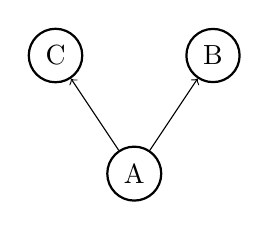
\begin{tikzpicture}[scale=0.5]
            \begin{scope}[every node/.style={circle,thick,draw}]
                \node (A) at (0,0) {A};
                \node (B) at (2,3) {B};
                \node (C) at (-2,3) {C};
            \end{scope}

            \begin{scope}
                \path [->] (A) edge node {} (B);
                \path [->] (A) edge node {} (C);
            \end{scope}
            \end{tikzpicture}
          \captionsetup{labelformat=empty}
          \caption{$\{\emptyset\}$}
        \end{subfigure}
        \begin{subfigure}{.15\textwidth}
            \centering
            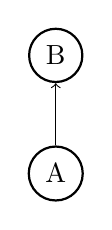
\begin{tikzpicture}[scale=0.5]
              \begin{scope}[every node/.style={circle,thick,draw}]
                  \node (A) at (0,0) {A};
                  \node (B) at (0,3) {B};
              \end{scope}

              \begin{scope}
                  \path [->] (A) edge node {} (B);
              \end{scope}
              \end{tikzpicture}
            \captionsetup{labelformat=empty}
            \caption{$\{\emptyset\}$}
          \end{subfigure}
        \begin{subfigure}{.15\textwidth}
          \centering
          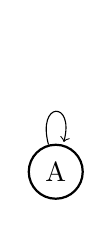
\begin{tikzpicture}[scale=0.5]
            \begin{scope}[every node/.style={circle,thick,draw}]
                \node (A) at (0,-0.3) {A};
                \node[draw=white] (B) at (0,3) {};
            \end{scope}

            \begin{scope}
                \path [->] (A) edge [loop above] node {} (A);
            \end{scope}
            \end{tikzpicture}
          \captionsetup{labelformat=empty}
          \caption{$A = \{A\}$}
        \end{subfigure}
        \begin{subfigure}{.25\textwidth}
            \centering
            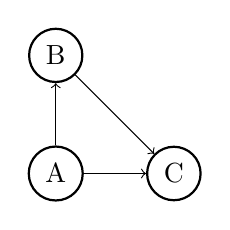
\begin{tikzpicture}[scale=0.5]
              \begin{scope}[every node/.style={circle,thick,draw}]
                  \node (A) at (0,0) {A};
                  \node (B) at (0,3) {B};
                  \node (C) at (3,0) {C};
              \end{scope}

              \begin{scope}
                  \path [->] (A) edge node {} (B);
                  \path [->] (B) edge node {} (C);
                  \path [->] (A) edge node {} (C);
              \end{scope}
              \end{tikzpicture}
            \captionsetup{labelformat=empty}
            \caption{$\{\emptyset, \{\emptyset\}\}$}
          \end{subfigure}

        \caption{Rappresentazione di insiemi tramite grafi}
        \label{fig:graph_set}
    \end{figure}
    In Figura \ref{fig:graph_set} sono rappresentati alcuni insiemi sotto forma di APG.
\end{example}

\subsection{Bisimulazione}
In questa sezione introdurremo la definizione di bisimulazione ed alcune proprietà immediate. In seguito esamineremo la relazione tra la teoria degli insiemi e la bisimulazione.
\subsubsection{Definizione e risultati generali}
\begin{definition}
    Siano $G_1 = (V_1,E_1), G_2 = (V_2,E_2)$ due grafi diretti. Una relazione binaria $R: V_1 \times V_2$ è una \emph{bisimulazione} su $G_1, G_2$ se $\forall a \in V_1, b \in V_2$ valgono congiuntamente le seguenti proprietà:
    \begin{itemize}
        \item $a R b, a E_1 a' \implies \exists b' \in V_2 \mid (a' R b' \land b E_2 b')$
        \item $a R b, b E_2 b' \implies \exists a' \in V_1 \mid (a' R b' \land a E_1 a')$
    \end{itemize}
    Analogamente si definisce una bisimulazione su un unico grafo diretto $G$, ponendo $G_1 = G_2 = G$.
\end{definition}
L'esistenza di una bisimulazione tra due grafi, come vedremo, è un'informazione rilevante se siamo interessati agli insiemi rappresentati dai grafi considerati:
\begin{definition}
    Siano $G_1 = (V_1,E_1), G_2 = (V_2,E_2)$ due grafi. Essi sono \emph{bisimili} se esiste una bisimulazione su $G_1, G_2$.\\
    Due APG $(G_1, v_1), (G_2, v_2)$ sono \emph{bisimili} se $G_1, G_2$ sono bisimili e vale $v_1 R v_2$ per almeno una bisimulazione $R$ su $G_1, G_2$.
\end{definition}
\begin{observation}
    Una bisimulazione può non essere riflessiva, simmetrica, nè transitiva.
\end{observation}
\begin{example}
    La relazione $a R b \iff$ ``$a,b$ sono lo stesso nodo'' su un grafo qualsiasi è una bisimulazione riflessiva, simmetrica e transitiva.\\
    La relazione $R = \emptyset$ è una bisimulazione su un grafo qualsiasi, ma non è riflessiva.\\
    La relazione $R = \{(a,a),(b,b),(c,c),(d,d),(a,b),(b,c),(c,d)\}$ sul grafo $G = (\{a,b,c,d\}, \{(a,b),(b,c),(c,d),(d,d)\})$ è una bisimulazione, ed è solamente riflessiva.
\end{example}
Dalla definizione di bisimulazione possiamo dedurre una proprietà interessante delle chiusure:
\begin{theorem}
    Sia $R$ una bisimulazione sul grafo diretto $G$. La sua chiusura riflessiva, simmetrica o transitiva è ancora una bisimulazione su $G$.
\end{theorem}
\begin{proof2}
    Consideriamo separatamente le tre relazioni $R_r, R_s, R_t$, rispettivamente la chiusura riflessiva, simmetrica e transitiva:
    \begin{itemize}
        \item $R_r$: Per definizione $R \subset R_r$, quindi è sufficiente dimostrare che $R_r$ è una bisimulazione quando gli argomenti $u,v \in V$ non sono distinti.\\
        Sia $u \in V$. Chiaramente per definizione di $R_r$ si ha $u R_r u$. Se $\exists u' \in V \mid u E u'$ allora (sempre per definizione di $R_r$) si ha $u' R_r u'$.
        \item $R_s$: Per definizione $R \subset R_s$, quindi è sufficiente dimostrare che $R_s$ è una bisimulazione quando per $u,v \in V$ si ha $u R v$ ma non $v R u$.\\
        Sia $(u,v) \in V\times V$. Allora:
        \begin{center}
            $u R_s v \implies u R v \lor v R u$
        \end{center}
        Supponiamo ad esempio che $v R u$.
        \begin{align*}
            &\implies \forall v' \in V\mid (v E v') \,\,\exists u' \in V, (u E u' \land v' R u')\\
            &\implies u' R_s v'
        \end{align*}
        e
        \begin{align*}
            &\implies \forall u' \in V\mid (u E u') \,\,\exists v' \in V, (v E v' \land v' R u')\\
            &\implies u' R_s v'
        \end{align*}
        cioè sono dimostrate le due condizioni caratteristiche della bisimulazione.\\
        La dimostrazione è analoga se $u R v$.
        \item $R_t$: Per definizione $b \subset R_t$, quindi è sufficiente dimostrare che $R_t$ è una bisimulazione quando per gli argomenti $u,v,z \in V$ si ha $u R v$, $v R z$ ma non $u R z$.\\
        Sia $(u,v,z) \in V\times V\times V$ con questa proprietà. Allora:
        \begin{gather*}
            \forall u' \in V\mid u E u' \,\, \exists v' \in V, (v E v' \land u' R v')
        \end{gather*}
        Inoltre $\exists z' \mid z E z' \land v' R z'$.\\
        Riordinando si ha $u' R v', v' R z'$. Allora per definizione di $b_t, \, u' R_t z'$.\\
        In modo speculare si ottiene la seconda condizione caratteristica della bisimulazione.
    \end{itemize}
    \vspace*{-0.75cm}
\end{proof2}
Da questa proposizione si deduce il seguente corollario, che risulta dall'applicazione iterata delle tre chiusure viste in precedenza:
\begin{corollary}
    Ad ogni bisimulazione $R$ è possibile associare una bisimulazione $\widetilde{R} : R \subset \widetilde{R} \,\,\land\,\, \widetilde{R}$ è una relazione di equivalenza.
    \label{cor:bisimulation_eqrel}
\end{corollary}
Concludiamo la sezione relativa ai risultati generali sulla bisimulazione con la seguente proposizione, che sarà utile nel seguito:
\begin{proposition}
    Siano $R_1, R_2$ due bisimulazioni su $G_1, G_2$. Allora $R = R_1 \cup R_2$ è ancora una bisimulazione.
    \label{obs:bisimulation_union}
\end{proposition}
\begin{proof2}
    Siano $u,v \mid u R v$. Sia $u' \mid u E u'$. Allora deve essere $u R_1 v \lor u R_2 v$. Ma quindi $\exists v' \mid (v E v' \land u' R_{1|2} v')$.
\end{proof2}

\subsubsection{Bisimulazione massima}
\label{sec:bisi_max}
Definiamo ora il concetto di \emph{bisimulazione massima}, che gioca un ruolo chiave nella risoluzione dei problemi considerati in questo elaborato:
\begin{definition}
    Una bisimulazione $R_M$ su $G_1, G_2$ è \emph{massima} se per ogni bisimulazione $R$ su $G_1,G_2 \,\, u R v \implies u R_M v$.
\end{definition}
\begin{observation}
    Sia $R_M$ la bisimulazione massima su un grafo diretto $G$. Allora per qualsiasi altra bisimulazione $R$ su $G$ si ha $|R_M| \geq |R|$.
\end{observation}
Naturalmente la bisimulazione massima dipende dai due grafi presi in esame. Possiamo dedurre alcune caratteristiche banali:
\begin{proposition}
    Valgono le seguenti proprietà:
    \begin{enumerate}
        \item La bisimulazione massima su due grafi $G_1,G_2$ è unica;
        \item La bisimulazione massima è una relazione di equivalenza.
    \end{enumerate}
    \vspace*{-0.3cm}
    \label{prop:bisi_max_equi}
\end{proposition}
\begin{proof2}
    Le proprietà seguono dal Corollario \ref{cor:bisimulation_eqrel} e dall'Osservazione \ref{obs:bisimulation_union}:
    \begin{enumerate}
        \item Supponiamo per assurdo che esistano due bisimulazioni massime $R_{M_1}, R_{M_2}$. La loro unione è ancora una bisimulazione, che è "più massima" delle supposte bisimulazioni massime.
        \item Se per assurdo la bisimulazione massima non fosse una relazione di equivalenza, potremmo considerare la sua chiusura riflessiva, simmetrica e transitiva, che avrebbe cardinalità maggiore o uguale, e sarebbe per costruzione una relazione di equivalenza.
    \end{enumerate}
    \vspace*{-0.7cm}
\end{proof2}
Naturalmente il concetto di \emph{bisimulazione massima} può essere definito anche su unico grafo diretto $G$. Questo caso si rivelerà di grande interesse nel seguito. Per ora dimostriamo il seguente risultato:
\begin{theorem}
    Sia $G$ un grafo diretto finito. Allora esiste la bisimulazione massima su $G$.
\end{theorem}
\begin{proof2}
    Può esistere solamente un numero finito di relazioni binarie su $G$, e questo numero fornisce un limite superiore al numero massimo di bisimulazioni su $G$.
    Allora possiamo considerare l'unione di questo numero finito di bisimulazioni, che sarà chiaramente la bisimulazione massima.
\end{proof2}

\subsubsection{Interpretazione insiemistica della bisimulazione}
Mostriamo ora una conseguenza diretta dell'Assioma di Estensionalità e di AFA:
\begin{theorem}
    Due APG rappresentano lo stesso insieme $\iff$ sono bisimili.
    \label{theo:bisi_iff_eqsets}
\end{theorem}
\begin{proof2}
    Siano $G_A = (V_A, E_A), G_B = (V_B, E_B)$. Dimostriamo separatamente le due implicazioni:
    \begin{enumerate}
        \item[$(\implies)$] Osserviamo innanzitutto che la relazione binaria ``$\equiv$'' su $V_A, V_B$ definita come segue:
              \begin{gather*}
                  a \equiv b \iff ``\text{le decorazioni di } A,B \text{ associano ad } a,b \text{ lo stesso insieme}''
              \end{gather*}
              è una bisimulazione sui grafi $G_A, G_B$.\\
              Chiaramente se $a \equiv b, a E a'$ si ha:
              \begin{itemize}
                  \item $a' \in a$, associando ad $a,a'$ gli insiemi che rappresentano secondo la decorazione (l'unica) considerata;
                  \item $a,b$ rappresentano lo stesso insieme.
              \end{itemize}
              Quindi per l'Assioma di Estensionalità $\exists b' \in b\mid b' = a'$, cioè $b E b'$ e $a' \equiv b'$. Si procede specularmente per la seconda condizione caratteristica della bisimulazione.\\
              La relazione ``$\equiv$'' è una bisimulazione sugli APG $G_A,G_B$ quando si assume per ipotesi che rappresentino lo stesso insieme.
        \item[$(\impliedby)$] Sia $R$ una bisimulazione su $G_A,G_B$. Consideriamo la decorazione $d_A$ (l'unica) di $G_A$. Vogliamo estrapolarne una decorazione per $G_B$, e dimostrare che i due grafi con le rispettive decorazioni sono due immagini dello stesso insieme. Dalla possibilità di operare questo procedimento, dall'Assioma di Estensionalità e da AFA potremo dedurre l'uguaglianza degli insiemi rappresentati.\\
              Definiamo la decorazione $d_B$ come segue:
              \begin{gather*}
                  d_B(v) = d_A(u), \text{con $u$ nodo di $G_A$} \mid u R v
              \end{gather*}
              \begin{observation*}
                  Per ogni nodo $v$ di $B$ deve esistere almeno un nodo $u$ di $G_A \mid u R v$ perchè si suppone che i due APG siano bisimili.
              \end{observation*}
              Dimostriamo che $d_B$ è una decorazione di $G_B$. In altre parole vogliamo dimostrare che per ogni nodo $v$ di $G_B$ l'insieme $d_B(v)$ contiene tutti e soli gli insiemi $d_B(v')$ dove $v'$ è figlio di $v$.
              \begin{itemize}
                  \item Supponiamo per assurdo che tra i figli di $v$ ``manchi" il nodo corrispondente ad un elemento $X \in d_B(v)$. Poichè la decorazione di $G_A$ è ben definita,il nodo $u$ di $G_A \mid u R v$ deve avere un figlio corrispondente a $X$, che chiameremo $u'$. Ma $u R b, u E u' \implies \exists v' \mid v E v', u' R v'$. Cioè $d_B(v') = X$. Dunque il nodo mancante è stato identificato.
                  \item Supponiamo per assurdo che tra i figli di $v$ ci sia un nodo ``in più'', ovvero un nodo $v' \mid v E v', d_B(v') = Y$ con $Y \notin d(v)$. Ma allora, sempre considerando $u$ il nodo di $G_A \mid u R v$, dovrebbe esistere un $u' \mid u E u', u' R v'$, cioè $d_A(u') = d_B(v') = Y$.
                  Ma allora $Y \in d_A(u) = d_B(v)$, deduzione che è chiaramente in contrasto con l'ipotesi.
              \end{itemize}
              E' possibile che ci siano due nodi di $a_1, a_2$ di $G_A$ ed un nodo $b$ di $G_B$ per cui vale $a_1 R b \land a_2 R b$. In questo caso la decorazione definita è ambigua. Per questo motivo correggiamo la formulazione di $d_B$ come segue:
              \begin{gather*}
                d_B(v) = X \text{, dove $X$ è l'insieme associato al nodo $u$ di $A$} \mid u R v, \\
                \text{con $u$ preso casualmente tra i nodi di $G_A$ bisimili a $v$.}
              \end{gather*}
              Per AFA esiste un'unica decorazione di $G_B$, quindi si deve avere, alternativamente, per ogni nodo $v$ di $G_B$:
              \begin{itemize}
                  \item $\exists ! u$ nodo di $G_A \mid u R v$;
                  \item $\forall u$ nodo di $G_A \mid u R v$, la decorazione di $G_A$ associa a tutti gli $u$ lo stesso insieme.
              \end{itemize}
              Dunque l'ambiguità è risolta.
    \end{enumerate}
    \vspace*{-0.75cm}
\end{proof2}
Tenendo conto di quanto affermato nella sezione \ref{sec:graphs_sets}, il Teorema \ref{theo:bisi_iff_eqsets} dimostra che la bisimulazione può sostituire la relazione di uguaglianza tra insiemi quando questi sono rappresentati con APG \cite{dovier}.\\

Dopo questa considerazone possiamo dare la seguente definizione:
\begin{definition}
    \label{def:bisi_contraction}
    Sia $R$ una bisimulazione su $G = (V,E)$, dove $G$ è un grafo diretto. Supponiamo che $R$ sia una relazione di equivalenza. Il grafo, definito a partire dal grafo iniziale, ottenuto con una \emph{contrazione rispetto alla bisimulazione} $R$, è il grafo diretto $G_R = (V_R, E_R)$ definito come in \cite{gentilini}:
    \begin{itemize}
        \item $V_R = \{[m]_R, m \in V\}$;
        \item $[m]_R E_R [n]_R \iff \exists b \in [m]_R, c \in [n]_R \mid b E c$.
    \end{itemize}
    Si chiama \emph{classe} del nodo $a$ rispetto alla bisimulazione $R$, indicata con la notazione $[a]_R$, il nodo di $V_R$ in cui viene inserito il nodo $a$.
\end{definition}
La Definizione \ref{def:bisi_contraction} è di fondamentale importanza per la seguente osservazione:
\begin{proposition}
    Sia $G$ un grafo diretto, e sia $G_R$ come nella Definizione \ref{def:bisi_contraction}, per una bisimulazione $R$ qualsiasi. Allora $G, G_R$ sono bisimili.
    \label{prop:bisi_cont_bisi}
\end{proposition}
\begin{proof2}
    Sia ``$\equiv$'' la relazione binaria su $V\times V_R$ definita come segue:
    \begin{gather*}
        m \equiv M \iff M = [m]_R
    \end{gather*}
    Vogliamo dimostrare che tale relazione è una bisimulazione sui grafi $G, G_R$.\\
    Supponiamo che $x \equiv X$, e che $x E y$ per qualche $y \in V$. Chiamiamo $Y \coloneqq [y]_R$. Allora, per la Definizione \ref{def:bisi_contraction}, si ha $X E_R Y$. Inoltre vale banalmente $y \equiv Y$.\\
    Per dimostrare la seconda condizione caratteristica della bisimulazione, supponiamo che $x \equiv X$, e che $X E_R Y$ per qualche $Y \in V_R$. Sempre per la Definizione \ref{def:bisi_contraction} deve esistere un $y \in Y \mid (y \equiv Y \land x E y)$.
\end{proof2}
La Proposizione \ref{prop:bisi_cont_bisi} ha una conseguenza ovvia, che risulta evidente dal Teorema \ref{theo:bisi_iff_eqsets}:
\begin{corollary}
    Sia $R$ una bisimulazione che sia anche una relazione di equivalenza. Allora l'APG $(G, v)$ e l'APG $(G_R, [v]_R)$ rappresentano lo stesso insieme.
\end{corollary}
Quindi risulta naturale sfruttare le proprietà della bisimulazione per minimizzare la rappresentazione di insiemi, considerando che è sufficiente una bisimulazione sulla rappresentazione iniziale per ottenere una rappresentazione equivalente. Definiamo una relazione d'ordine sulle rappresentazioni:
\begin{definition}
    La rappresentazione $(G_a, v_a)$ di un insieme è \emph{minore} della rappresentazione equivalente $(G_b, v_b)$ se $|Va| < |Vb|$.\\
    Una rappresentazione è \emph{minima} se non esiste una rappresentazione equivalente minore.
\end{definition}
\begin{observation}
    La \emph{contrazione per bisimulazione} è una rappresentazione minore (o eventualmente uguale) di quella iniziale.
\end{observation}
Concludiamo la sezione con il seguente risultato, che stabilisce in modo univoco la bisimulazione prescelta per minimizzare la rappresentazione di un dato insieme:
\begin{theorem}
    Sia $(G,v)$ un APG rappresentante un insieme. Sia $R_M$ la bisimulazione massima su $(G,v)$. Allora la contrazione per bisimulazione indotta da $R_M$ su $(G,v)$ fornisce la rappresentazione minima dell'insieme.
\end{theorem}
\begin{proof2}
    Supponiamo per assurdo che esista una bisimulazione $R_V$ su $(G,v)$ che fornisce una contrazione avente un numero di nodi strettamente inferiore alla contrazione indotta da $R_M$. Ma questo implica che esistono almeno due nodi di $G$ che sono in relazione secondo $R_V$ e non secondo $R_M$. Chiaramente questa deduzione è in contrasto con il fatto che $R_M$ è la bisimulazione massima.\\
    Supponiamo per assurdo che, dopo la contrazione indotta da $R_M$, sia possibile trovare una nuova bisimulazione $R_O$ su $(G_{R_M}, [v]_{R_M})$ che induca una contrazione avente un numero di nodi strettamente inferiore a quello di $(G_{R_M}, [v]_{R_M})$. Chiaramente $R_O \subset V{R_M} \times V{R_M}$.\\
    Definiamo una nuova bisimulazione $R_{\widetilde{M}} \subset V\times V$ tale che
    \begin{gather*}
        x R_{\widetilde{M}} y \iff (x R_M y \lor [x]_{R_M} R_O [y]_{R_M})
    \end{gather*}
    Per definizione di bisimulazione massima bisogna avere $R_{\widetilde{M}} \subset R_M$, quindi non è possibile che la contrazione indotta da $R_O$ sia una rappresentazione minore di quella indotta da $R_M$.
\end{proof2}

\subsection{Relational stable coarsest partition}
\label{sec:rscp}
In questa sezione introdurremo il concetto di \emph{RSCP} o \emph{Relational Stable Coarsest Partition}. Nel seguito del lavoro evidenzieremo il legame tra questo problema e quello della determinazione della bisimulazione massima, sfruttato ampiamente dagli algoritmi che tratteremo nel seguito in quanto la formulazione del primo lo rende un problema più facilmente approcciabile dal punto di vista algoritmico.\\
Cominciamo con alcune definizioni di base:
\begin{definition}
    Sia $S$ un insieme finito. Sia $X = \{x_1, \dots, x_n\}$ con $x_i \subseteq S \,\,\,\forall i \in \{1,\dots,n\}$. $X$ è una \emph{partizione} di $S$ se:
    \begin{gather*}
        \bigcup_{i = 1}^n x_i = A \qquad \land \qquad x_i \cap x_j = \emptyset \,\,\forall i,j \in \{1,\dots,n\} \qquad \land \qquad x_i \neq \emptyset \,\,\forall i
    \end{gather*}
    Inoltre gli insiemi $x_i$ sono i \emph{blocchi} della partizione $X$. Se $a \in x_i$ si usa la notazione $[a]_X = x_i$.
\end{definition}
\begin{observation}
    \label{obs:part_banale}
    Ogni insieme $S$ ha una partizionamento banale, consistente in un unico blocco contenente tutti gli elementi dell'insieme.
\end{observation}
\begin{example}
    Sia $S \coloneqq \{0,1,2,3,4,5,6\}$. Alcuni possibili partizionamenti sono $\{S\}$ (il partizionamento banale), $S_1 = \{\{0,1,2,3\},\{4,5,6\}\}, S_2 = \{\{0,1\},\{2,3\},\{4,5,6\}\}$.
    \label{exa:set_partition}
\end{example}
\begin{definition}
    Siano $X_1,X_2$ due partizioni dello stesso insieme. $X_2$ \emph{rifinisce} $X_1$ se $\forall x_2 \in X_2, \,\,\exists x_1 \in X_1 \mid x_2 \subseteq x_1$.
\end{definition}
\begin{example}
    Riprendendo l'Esempio \ref*{exa:set_partition}, la partizione $S_2$ rifinisce $S_1$, che a sua volta rifinisce la partizione banale.
\end{example}
Il partizionamento di insiemi finiti assume interesse nell'ambito trattato in questo lavoro quando si impone la seguente condizione sui blocchi:
\begin{definition}
    Sia $S$ un insieme, ed $R$ una relazione binaria su $S$. Sia $X$ una partizione su $S$, e sia $B \subseteq A$.
    \begin{itemize}
        \item $X$ è \emph{stabile} rispetto alla coppia $(B,R)$ se $\forall x \in X$ vale $x \subseteq R^{-1}(B) \lor x_i \cap R^{-1}(B) = \emptyset$;
        \item La partizione $X$ è \emph{stabile} rispetto ad $R$ se è stabile rispetto a $(x,R) \,\,\forall x \in X$.
    \end{itemize}
\end{definition}
\begin{example}
    \label{exa:set_partition_stable}
    Consideriamo la relazione binaria $R$ su $S$ che mette in relazione le coppie $\{(0,1),(1,0),(2,3),(3,2),(4,5),(5,6),(0,4),(1,5)\}$. $S_2$ è stabile rispetto a $R$, ma lo stesso non vale per $S_1$.
\end{example}
In altre parole per ogni coppia di blocchi di una partizione stabile si hanno due alternative:
\begin{itemize}
    \item Tutti gli elementi del primo blocco sono in relazione con almeno un elemento del secondo blocco;
    \item Nessuno degli elementi del primo blocco è in relazione con qualche elemento del secondo blocco.
\end{itemize}
Vale il seguente risultato:
\begin{proposition}
    Sia $\widetilde{S}$ una partizione qualsiasi di un insieme $S$, e siano $P,Q \subseteq S$. Sia $R$ una relazione binaria su $S$. Supponiamo $\widetilde{S}$ stabile rispetto alle coppie $(R,P),(R,Q)$. Allora:
    \begin{enumerate}
        \item Qualsiasi rifinitura di $\widetilde{S}$ resta stabile rispetto alla coppia $(R,P)$;
        \item $\widetilde{S}$ è stabile rispetto alla coppia $(f,P \cup Q)$.
    \end{enumerate}
\end{proposition}
\begin{proof2}
    Dimostriamo separatamente i due enunciati:
    \begin{enumerate}
        \item Chiaramente se per un blocco qualsiasi $x \in X$ vale $x \subseteq R^{-1}(P) \lor x \cap R^{-1}(P) = \emptyset$, la stessa relazione vale per qualsiasi sottoinsieme di $x$;
        \item Sia $x \in S$. Chiaramente vale $R^{-1}(P),R^{-1}(Q) \subseteq R^{-1}(P \cup Q)$. Allora, se almeno uno tra $R^{-1}(P),R^{-1}(Q)$ contiene l'immagine di $x$ si avrà $x \subseteq R^{-1}(P \cup Q)$, altrimenti $x \cap R^{-1}(P \cup Q)$ dovrà chiaramente essere vuoto.
    \end{enumerate}
    \vspace*{-0.75cm}
\end{proof2}
\accente evidente che l'ultimo punto può essere esteso in modo molto semplice all'unione di più sottoinsiemi di $S$. In altre parole, se $\widetilde{S}$ è stabile rispetto alle coppie $(R,S_i), S_i \subset S, i = 1, \dots, n$, allora è stabile anche rispetto alla coppia $(R, \bigcup_{i=1}^{n} S_i)$.

Con queste premesse possiamo definire il problema della determinazione della RSCP:
\begin{definition}
    Sia $S$ un insieme, sia $R$ una relazione binaria su $S$. Sia $\widetilde{S}$ una partizione di $S$. La $\rscp(\widetilde{S},R)$ di $S$ è la partizione di $S$ stabile rispetto ad $R$, che rifinisce $\widetilde{S}$ e che contiene il minor numero di blocchi (per questo motivo si dice che è la \emph{più rozza}).\\
    Si usa la notazione ``$\rscp(R)$'' se la partizione iniziale è quella banale proposta nella Definizione \ref{obs:part_banale}.
\end{definition}
\begin{example}
    Riprendendo l'Esempio \ref*{exa:set_partition_stable}, è evidente che la $\rscp(R)$ deve avere almeno due blocchi: infatti ``6'' non è in relazione con nessun elemento, dunque deve essere posto in un blocco a parte. La RSCP è quindi $\{\{0,1,2,3,4,5\},\{6\}\}$.
\end{example}

\subsubsection{Insiemi \emph{splitter}, e la funzione Split}
La seguente definizione ha grande importanza pratica per il problema della determinazione della RSCP:
\begin{definition}
    \label{def:funz_split}
    Sia $\widetilde{S} = \{S_1,\dots,S_n\}$ una partizione qualsiasi di un insieme finito $S$. Sia $f: S \to S$, e sia $A \subset S$. $A$ è uno \emph{splitter} di $S$ rispetto a $f$ se
    \begin{gather*}
        \exists S_x \in \widetilde{S} \mid \,\, S_x \cap f^{-1}(A) \neq \emptyset \,\,\land\,\, S_x \not\subseteq f^{-1}(A)
    \end{gather*}
    ovvero se la partizione non è stabile rispetto ad $A$. In tal caso definiamo la seguente funzione:
    \begin{gather*}
        \splitfunc(A,\widetilde{S}) = \{S_x \cap f^{-1}(A), S_x - f^{-1}(A) \mid S_x \in \widetilde{S}\} - \{\emptyset\}
    \end{gather*}
\end{definition}
Valgono i seguenti risultati sulla funzione appena introdotta:
\begin{observation}
    Se $A$ non è uno \emph{splitter} di $\widetilde{S}$ si ha $\widetilde{S} = \splitfunc(A,\widetilde{S})$.
\end{observation}
\begin{proposition}
    \label{prop:split_eredita}
    Se $\widetilde{S}$ è stabile rispetto ad un insieme $A, \splitfunc(B,\widetilde{S})$ è stabile rispetto ad $A,B$. In altre parole la funzione ``Split'' preserva la stabilità.
\end{proposition}
\begin{proof2}
    ``Split'' può solamente dividere i blocchi, e non mescolarli.
\end{proof2}
Dimostriamo il seguente risultato che useremo nel seguito:
\begin{theorem}
    \label{theo:split_properties}
    Consideriamo la funzione ``Split'' proposta nella Definizione \ref{def:funz_split}:
    \begin{enumerate}
        \item La funzione è monotona rispetto al secondo argomento, cioè se $\widetilde{S}$ rifinisce di $S$, allora $\splitfunc(A,\widetilde{S})$ rifinisce $\splitfunc(A,S)$;
        \item La funzione è commutativa rispetto al primo argomento: \splitfunc$(A,\splitfunc(B,S)) = \splitfunc(B, \splitfunc(A,S))$.
    \end{enumerate}
\end{theorem}
\begin{proof2}
    Dimostriamo separatamente gli enunciati:
    \begin{enumerate}
        \item I blocchi di \splitfunc$(A,\widetilde{S})$ sono del tipo $x - R^{-1}(A)$ oppure $x \cap R^{-1}(A)$, dove $x$ è un blocco di $\widetilde{S}$. I blocchi di \splitfunc$(A,S)$ sono del tipo $y - R^{-1}(A)$ oppure $y \cap R^{-1}(A)$, dove $y$ è un blocco di $S$. Poichè $\forall x \in \widetilde{S} \,\,\exists y \in S \mid x \subseteq y$ si ha $x - R^{-1}(A) \subseteq y - R^{-1}(A)$ e $x \cap R^{-1}(A) \subseteq y \cap R^{-1}(A)$;
        \item Conseguenza della commutatività delle operazioni ``$-$'' e ``$\cap$'' su insiemi.
    \end{enumerate}
    \vspace*{-0.75cm}
\end{proof2}

\subsection{Equivalenza tra RSCP e bisimulazione massima}
Dimostriamo innanzitutto il seguente risultato preliminare presentato in \cite{gentilini}:
\begin{proposition}
    Sia $G = (V,E)$. Sia $X$ una partizione di $V$ stabile rispetto a $E$. Allora la relazione binaria $R$ su $V$ definita come:
    \begin{gather*}
        a R b \iff [a]_X = [b]_X
    \end{gather*}
    è una bisimulazione su $G$.
    \label{prop:part_induce_bisi}
\end{proposition}
\begin{proof2}
    Siano $a,b \in G \mid a R b$, e sia $a' \mid a E a'$. Poichè $X$ è stabile, si ha che $[a]_X \subseteq E^{-1}([a']_X)$. Quindi $\exists b' \in [a']_X \mid b E b'$.\\
    L'altra condizione caratteristica della bisimulazione si dimostra in modo speculare.
\end{proof2}
In altre parole, una qualsiasi partizione stabile rispetto a $E$ induce su un grafo diretto una bisimulazione che può essere ricavata in modo banale.\\
Dimostriamo ora il risultato opposto:
\begin{proposition}
    Sia $R$ una bisimulazione su $G$ che sia anche una relazione di equivalenza. Allora la partizione i cui blocchi sono le classi di equivalenza di $R$ è stabile rispetto a $E$.
    \label{prop:bisi_induce_part}
\end{proposition}
\begin{proof2}
    Se per assurdo $X$ non fosse stabile esisterebbero due blocchi $x_1, x_2 \mid x_1 \,\,\cap E^{-1}(x_2)$ non è ne $x_1$ nè $\emptyset$. Chiamiamo $A$ questo insieme.\\
    Gli elementi $a$ di $A$ sono i nodi in $x_1 \mid \nexists b \in x_2$ per cui valga $a E b$. Ma poichè questi $a$ e gli $x \in x_1 - A$ si trovano all'interno dello stesso blocco $x_1$ deve valere $x R a$.\\
    Sia $x \in x_1 - A$, ed $y \in x_2 \mid x E y$. Poichè $\forall a \in A$ vale $x R a$, allora $\exists a' \mid a E a', a' R y$, cioè $[a']_X = [y]_X = x_2$. Quindi $A$ deve necessariamente essere vuoto.
\end{proof2}
Cioè una bisimulazione induce un partizionamento stabile rispetto a $E$ dei nodi del grafo. Vale il seguente corollario:
\begin{corollary}
    Determinare la bisimulazione massima su un grafo diretto $G = (V,E)$ e trovare $\rscp(E)$ di $V$ sono problemi equivalenti.
\end{corollary}
\begin{proof2}
    Dimostriamo separatamente che la bisimulazione ricavata dalla $\rscp(E)$ è massima, e che la partizione ricavata dalla bisimulazione massima è la $\rscp(E)$.
    \begin{itemize}
        \item Sia $R_M$ la bisimulazione massima su $G$. Per la Proposizione \ref{prop:bisi_max_equi} è una relazione di equivalenza. Per la Proposizione \ref{prop:bisi_induce_part} è possibile determinare una partizione $X$ stabile rispetto a $E$.\\
              Supponiamo per assurdo che $X$ non sia $\rscp(E)$ di $V$, quindi esiste una partizione $\widetilde{X}$ stabile rispetto a $E$ che ha meno blocchi di quanti ne ha $X$. Ma per la Proposizione \ref{prop:part_induce_bisi} da
              $\widetilde{X}$ è possibile ricavare una bisimulazione $\widetilde{R}$ su $G$. Ma quindi $|\widetilde{R}| > |R|$, che è assurdo.
        \item Sia $X$ la $\rscp(E)$ di V. Supponiamo per assurdo che la bisimulazione $R$ ricavata da $X$ come nella Proposizione \ref{prop:part_induce_bisi} non sia massima. Allora deve esistere un'altra bisimulazione $\widetilde{R}$ che
              sia massima. Ma da questa si può ricavare, come nella Proposizione \ref{prop:bisi_induce_part}, una partizione $\widetilde{X}$ stabile rispetto a $E$ per cui vale $|\widetilde{X}| \leq |X|$. Ma questo è assurdo.
    \end{itemize}
    \vspace*{-0.75cm}
\end{proof2}

\clearpage
\section{Algoritmi risolutivi}
In questa sezione esamineremo alcuni algoritmi risolutivi proposti per la risoluzione del problema della determinazione della massima bisimulazione su un grafo. Come risulterà evidente nel seguito viene sfruttata ampiamente l'equivalenza tra bisimulazione massima e RCSP dimostrata nella sezione precedente.

\subsection{Minimizzazione di automi a stati finiti}
Esaminiamo innanzitutto l'algoritmo risolutivo per una versione semplificata del problema della determinazione della bisimulazione massima, ovvero la minimizzazione di un'automa a stati finiti, presentato in \cite{hopcroft} nel 1971. Sebbene questa soluzione non sia generale, ha fornito alcuni spunti fondamentali per l'ideazione di algoritmi risolutivi più completi, che verranno presentati nel seguito del lavoro.

\subsubsection{Alcune nozioni fondamentali}
Innanzitutto definiamo il concetto di \emph{automa}, chiaramente centrale nella descrizione del problema:
\begin{definition}
    Consideriamo i seguenti oggetti:
    \begin{itemize}
        \item Un insieme finito $I$ detto \emph{insieme degli ingressi};
        \item Un insieme finito $S$ detto \emph{insieme degli stati}, ad ogni stato è associata un'unica uscita;
        \item Un insieme finito $F \subseteq S$ detto \emph{insieme degli stati finali};
        \item Una funzione $\delta: S \times I E S$ detta \emph{funzione di trasferimento}.
    \end{itemize}
    Chiameremo $A = (S,I,\delta,F)$ \emph{automa}. Useremo la notazione $Out(x)$ per indicare l'output corrispondente allo stato $x$.
\end{definition}
Possiamo rappresentare un'automa con una tabella degli stati, in cui ogni riga rappresenta uno stato, ogni colonna un ingresso, ed ogni cella contiene il nuovo stato del sistema quando, nel momento in cui il sistema si trova nello stato corrispondente alla riga, si inserisce l'ingresso corrispondente alla colonna.In alternativa possiamo utilizzare una rappresentazione grafica, in cui ogni stato è descritto da un cerchio contenente il nome dello stato, e le transizioni tra stati sono descritte da frecce, sulle quali viene specificato l'ingresso che ha innescato la transizione.\\
\begin{example}
    Nella Tabella \ref{fig:tab_automata} è rappresentato un'automa che cambia stato ($A E B$, $B E C$) solamente se l'ingresso è ``1'', e lo stato non è ``$C$''. In qualsiasi altro caso lo stato non cambia.
    \begin{table}[ht]
        \centering
        \begin{tabular}{ c | c c }
            \hline
            & 0 & 1\\
            \hline
            a[0] & a & b \\
            b[0] & b & c \\
            c[1] & c & c \\
            \hline
          \end{tabular}
        \caption{Rappresentazione tabellare di un'automa}
        \label{fig:tab_automata}
    \end{table}
    \label{exa:automata_tab}
\end{example}
\begin{example}
    Nella Figura \ref{fig:automata} è rappresentato lo stesso automa dell'Esempio \ref{exa:automata_tab}.
    \begin{figure}[hb]
        \centering
        \begin{tikzpicture}[->,>=stealth',shorten >=1pt,auto,node distance=3.5cm,
            scale = 1,transform shape]
            \node[state] (a) {$a[0]$};
            \node[state] (b) [right of=a] {$b[0]$};
            \node[state] (c) [right of=b] {$c[1]$};

            \path (a) edge              node {$1$} (b)
                  (b) edge              node {$1$} (c)
                  (a) edge [loop above]             node {$0$} (a)
                  (b) edge [loop above]             node {$0$} (b)
                  (c) edge [loop above]              node {$0/1$} (c);
        \end{tikzpicture}
        \caption{Rappresentazione grafica di un'automa}
        \label{fig:automata}
    \end{figure}
\end{example}
In alcuni automi è possibile individuare stati che ``si comportano in modo simile''. Informalmente, il sistema si comporta in modo simile quando riceve in input un ingresso qualsiasi, e si trova in uno degli stati presi in esame. Diamo un esempio di questa situazione:
\begin{example}
    \begin{figure}[b]
        \centering
        \begin{tikzpicture}[->,>=stealth',shorten >=1pt,auto,node distance=3.5cm,
            scale = 1,transform shape]
            \node[state] (a) {$a[0]$};
            \node[state] (b) [right of=a] {$b[1]$};
            \node[state] (c) [right of=b] {$c[1]$};

            \path (a) edge              node {$1$} (b)
                  (b) edge [bend right]             node {$1$} (c)
                  (c) edge [bend right]             node {$1$} (b)
                  (a) edge [loop above]             node {$0$} (a)
                  (b) edge [loop above]             node {$0$} (b)
                  (c) edge [loop above]             node {$0$} (c);
        \end{tikzpicture}
        \caption{Automa contenente stati equivalenti}
        \label{fig:automata_eq}
    \end{figure}
    Consideriamo gli stati dell'automa rappresentato graficamente nella Figura \ref{fig:automata_eq}. Supponiamo di accorpare gli stati $B,C$ in un unico stato, che chiamiamo $B'$. Se ci interessiamo solamente alla sequenza di output ed all'eventuale raggiungimento di uno stato finale, il nuovo automa risulta indistinguibile dal primo.
\end{example}
Proponiamo la definizione formale di equivalenza tra stati che viene utilizzata in \cite{hopcroft}. Nel seguito ne dedurremo un'altra, che consente di stabilire un parallelo con gli argomenti trattati nella Sezione \ref{sec:base}.
\begin{definition}
    \label{def:equivalent_states}
    Sia $I^*$ l'insieme di tutte le sequenze di input di lunghezza finita. Sia $\delta^* : S \times I^*$ la funzione di transizione ``iterata''. Diremo che due stati $x,y$ sono equivalenti (con la notazione ``$x \sim y$'') se e soltanto se valgono congiuntamente le seguenti condizioni:
    \begin{enumerate}
        \item $Out(x) = Out(y)$;
        \item $\forall i^* \in I^*,\,\, \delta^*(x,i^*) \in F \iff \delta^*(y,i^*) \in F$.
    \end{enumerate}
\end{definition}
\accente evidente che individuare g
li stati equivalenti consente di minimizzare il sistema, preservando al tempo stesso i risultati ottenuti. In questo lavoro non illustreremo cosa comporta questa definizione, e perchè è importante che per qualsiasi stringa di lunghezza finita si giunga ad uno stato finale partendo da due stati supposti equivalenti.
\begin{observation}
    La relazione ``$\sim$'' così definita è una relazione di equivalenza sull'insieme degli stati di un'automa.
\end{observation}
La seguente proposizione sarà utile per formulare il problema con la terminologia esposta nella Sezione \ref{sec:rscp}:
\begin{proposition}
    \label{prop:equivalent_states}
    Due stati $x,y$ sono equivalenti nel senso della definizione \ref{def:equivalent_states} se e solo se
    \begin{gather}
        \forall i \in I, \quad \delta(x,i) \sim \delta(y,i)
    \end{gather}
    e $Out(x) = Out(y)$.
\end{proposition}
\begin{proof2}
    Supponiamo che $\exists i \in I : \delta(x,i) \not\sim \delta(y,i)$. Allora, ad esempio:
    \begin{gather*}
        \exists i^* \in I^* : \delta^*(\delta(x,i),i^*) = \delta^*(x,ii^*) \in F, \,\, \delta^*(\delta(y,i),i^*) = \delta^*(y,ii^*) \notin F
    \end{gather*}
    Quindi, per l'esistenza della stringa $ii^*$ si ha $x \not\sim y$. La dimostrazione è speculare se $\exists i^* \in I^* : \delta^*(x,ii^*) \notin F, \delta^*(y,ii^*) \in F$.\\
    Ora supponiamo che valga la (1). E' chiaro che $\forall i^* \in I^*, \forall i \in I$ si ha che
    \begin{gather*}
        \delta^*(x,ii^*) \sim \delta^*(y,ii^*)
    \end{gather*}
    e quindi $x \sim y$.
\end{proof2}
\begin{proposition}
    La relazione ``$\sim$'' con la formulazione dell'Osservazione \ref{prop:equivalent_states} è una bisimulazione sull'insieme degli stati di un'automa, se si considera la relazione binaria $\displaystyle E \,\,\coloneqq \bigcup_{i \in I, x \in S} \{(x,\delta(x,i))\}$.
\end{proposition}
\begin{proof2}
    Supponiamo che $x \sim y$. Sia $x E x'$, cioè $\exists i \in I : x' = \delta(x,i)$. Sia $y' = \delta(y,i) \implies y E y'$. Allora, per l'Osservazione \ref{prop:equivalent_states}, $x' \sim y'$.\\
    Chiaramente lo stesso argomento vale in modo speculare.
\end{proof2}
Osserviamo che nella definizione di ``$E$'' si perde un'informazione importante, cioè il fatto che per $i \in I$ fissato $\delta_i(x) \coloneqq \delta(x,i)$ è una funzione, ovvero l'insieme immagine di ogni $x \in S$ ha cardinalità 1. L'algoritmo di Hopcroft sfrutta questa proprietà nel procedimento che consente di migliorare l'algoritmo banale che verrà discusso nel seguito del lavoro.\\
Possiamo definire la \emph{minimizzazione per stati equivalenti} di un'automa a stati finiti:
\begin{definition}\label{def:minim_eq_states}
    Sia $A = (S,I,\delta,F)$ un'automa. Chiameremo \emph{minimizzazione per stati equivalenti} l'automa $A = (\widetilde{S}, I, \widetilde{\delta}, \widetilde{F})$ dove
    \begin{itemize}
        \item $\widetilde{S} =$ ``l'insieme delle classi di equivalenza di $\sim$ su $S$'';
        \item $\widetilde{\delta} : (\widetilde{S} \times I) E \widetilde{S}, \quad \delta(i, x) = y \implies \widetilde{\delta}(i,\widetilde{x}) = \widetilde{y}$, dove $x,y \in S, i \in I$, e $\widetilde{x}, \widetilde{y} \in \widetilde{S}$ sono rispettivamente le classi di equivalenza di ``$\sim$'' a cui appartengono $x,y$;
        \item $\widetilde{F} =$ ``l'insieme delle classi di equivalenza di $\sim$ su $F$'';
    \end{itemize}
\end{definition}
Prima di concludere l'esposizione delle nozioni preliminari è necessario dimostrare un risultato interessante che lega il problema della minimizzazzione di un'automa a stati finiti con quanto è stato presentato nella sezione \ref{sec:rscp}. A questo scopo dimostriamo i seguenti lemmi, che consentono di dimostrare tale legame in modo agevole:
\begin{lemma}
    \label{lem:part_stab_stesso_blocco}
    Sia $A = (S,I,F,\delta)$ un'automa. Sia $\widehat{S}$ una partizione di $S$ stabile rispetto alle funzioni $\delta_i, \forall i \in I$. Allora $\forall (x,y) \in S \times S$ tali che $[x]_{\widehat{S}} = [y]_{\widehat{S}}$ si ha che $\forall i^* \in I^*$
    \begin{gather*}
        [\delta^*(x,i^*)]_{\widehat{S}} = [\delta^*(y,i^*)]_{\widehat{S}}
    \end{gather*}
\end{lemma}
\begin{proof2}
    Procediamo per induzione su $i^*$. Inizialmente i due stati si trovano nello stesso blocco. Ora supponiamo che dopo l'inserimento dell' $(n-1)$-esimo simbolo di $i^*$ i due stati $x_{n-1}, y_{n-1}$ in cui si trova l'automa appartengano ancora allo stesso blocco. La partizione è stabile rispetto alla funzione $\delta_i$, dove $i$ è l' $n$-esimo simbolo di $i^*$, quindi tutto il blocco $[x_{n-1}]_{\widehat{S}} = [y_{n-1}]_{\widehat{S}}\,\,$ è contenuto all'interno dell'insieme $\delta_i^{-1}([\delta_i(x_{n-1})]_{\widehat{S}}) = \delta_i^{-1}([x_n]_{\widehat{S}})$. Quindi $\delta_i(y_{n-1}) \in \delta_i^{-1}([x_n]_{\widehat{S}})$, e dunque si ha anche $[x_n]_{\widehat{S}} = [y_n]_{\widehat{S}}$.
\end{proof2}
\begin{lemma}
    \label{lem:part_stab_equiv}
    Sia $A = (S,I,F,\delta)$ un'automa. Sia $\widehat{S}$ una partizione di $S$ stabile rispetto alle funzioni $\delta_i, \forall i \in I$. Supponiamo inoltre che per $\widehat{S}$ valga la segente condizione:
    \begin{gather*}
        \forall (x,f) \in S \times F, \quad [x]_{\widetilde{S}} = [f]_{\widetilde{S}} \implies x \in F
    \end{gather*}
    Allora $\forall X \in \widehat{S}, \,\,\forall (x,y) \in X \times X$ si ha $x \sim y$.
\end{lemma}
\begin{proof2}
    Supponiamo per assurdo che in un blocco $X \in \widehat{S}$ esistano due stati $x,y$ non equivalenti. Allora deve esistere una stringa $i^* \in I^*$ tale che, ad esempio, $\delta^*(x,i^*) \in F \land \delta^*(y,i^*) \not\in F$. Ma per il Lemma \ref{lem:part_stab_stesso_blocco} $[\delta^*(x,i^*)]_{\widehat{S}} = [\delta^*(y,i^*)]_{\widehat{S}}$. Chiaramente questo è assurdo per la condizione supposta nell'ipotesi, quindi non possono esistere nello stesso blocco due stati non equivalenti.
\end{proof2}
Possiamo dimostrare il seguente risultato:
\begin{theorem}
    \label{theo:auto_mini_rscp}
    Sia $A$ un'automa a stati finiti. Supponiamo che in tale automa ad uno stato finale ed uno non finale non possa essere assegnato un output identico. La minimizzazione per stati equivalenti proposta nella Definizione \ref{def:minim_eq_states} è l'automa avente per stati i blocchi della partizione più grossolana stabile rispetto alle funzioni $\delta_i : S E S, \forall i \in I$.
\end{theorem}
\begin{proof2}
    Dimostriamo che la minimizzazione proposta nella Definizione \ref{def:minim_eq_states} è una partizione stabile rispetto alle funzioni $\delta_i$. Supponiamo per assurdo che $\exists i \in I : \widetilde{S}$ non è stabile rispetto a $\delta_i$. Quindi $\exists S_1, S_2 \in S :$
    \begin{gather*}
        S_1 \not\subseteq \delta_i^{-1}(S_2) \,\, \land \,\, S_1 \,\cap \,\delta_i^{-1}(S_2) \neq \emptyset
    \end{gather*}
    La prima porzione dell'espressione implica che $\exists s \in S_1 : \delta_i(s) \not\in S_2$. Ma questo è chiaramente in contrasto con l'Osservazione \ref{prop:equivalent_states}, perchè $\forall (u,v) \in S_1 \times S_1$ deve valere $\delta_i(u) \sim \delta_i(v)$, mentre è evidente che, poichè $S_1 \,\cap\, \delta_i^{-1}(S_2) \neq \emptyset$, c'è almeno una coppia che non soddisfa questa condizione.\\
    Ora supponiamo che la partizione $\widetilde{S}$ non sia la più grossolana stabile rispetto alle funzioni $\delta_i : S E S, \forall i \in I$. Ne deve esistere, quindi, una (stabile) più grossolana, che chiamiamo $\widetilde{S}$. Chiaramente si ha $|\widehat{S}| < |\widetilde{S}|$, e quindi devono esistere almeno due blocchi $S_1,S_2 \in \widetilde{S}$ ed un blocco $X \in \widehat{S}$ tali che
    \begin{gather*}
        S_1 \cap X \neq \emptyset \,\,\land\,\, S_2 \cap X \neq \emptyset
    \end{gather*}
    Ma questo è chiaramente in contrasto con il Lemma \ref{lem:part_stab_equiv} per come è stata costruita la partizione $\widetilde{S}$, in quanto esistono coppie di stati $(x,y) \in X \times X$ per cui vale $x \in S_1, y \in S_2$, cioè $x \not\sim y$.
\end{proof2}
Osserviamo che la condizione richiesta nell'ipotesi del Teorema \ref{theo:auto_mini_rscp}, che impone l'assegnazione di un output diverso a stati finali e non finali, è estremamente leggera: dato un'automa qualsiasi è sempre possibile costruirne un altro, che soddisfa tale condizione, in tempo lineare rispetto al numero di stati.

\subsubsection{L'algoritmo naive}
Innanzitutto, con i risultati della sezione precedente, possiamo progettare il seguente algoritmo banale:\\
\begin{algorithm}[H]
    \label{alg:hop_banale}
    \SetAlgoLined
    \KwData{$S,I,\delta$}
    \tcp*[h]{Partizione iniziale contenente un unico blocco}
    \nl$\widetilde{S} \coloneqq \{\{s_1, \dots, s_n\}\}$\;
    \tcc*[h]{Separiamo gli stati non equivalenti in base all'output}\\
    $\widetilde{S} = $ PartizionaPerOutput($\widetilde{S}$)\;\label{alg:hop_banale_partiziona_output}
    \ForAll{$i \in I$} {
        \label{alg:hop_banale_for_ingressi}
        \For{$NS = $ BlocchiNonStabili(S,$\delta_i$)), $NS \neq \emptyset$}{
            \label{alg:hop_banale_for_ns}
            \tcc*[h]{Estraiamo casualmente una coppia di blocchi non stabili}\\
            $(X,Y) = NS[0]$\;
            $X_1 \coloneqq X - \delta_i^{-1}({Y})$\;
            $X_2 \coloneqq X \cap \delta_i^{-1}({Y})$\;
            \tcp*[h]{Aggiorniamo $S$}\\
            $\widetilde{S} = (\widetilde{S} - \{X\}) \cup \{X_1,X_2\}$\;
        }
    }
    \Return{$S$}
    \caption{Procedimento banale per la minimizzazzione}
\end{algorithm}
L'algoritmo termina, perchè la condizione del ciclo diventa sicuramente falsa quando la partizione $S$ è composta da $n$ blocchi, uno per ogni stato, ed ad ogni iterazione un blocco viene diviso in due blocchi distinti e non vuoti. \\
Inoltre la risposta fornita è corretta, perchè l'algoritmo si ferma appena viene trovata una partizione stabile. Poichè ad ogni iterazione del ciclo definito nella Riga \ref{alg:hop_banale_for_ns} il numero di blocchi aumenta di 1, il risultato è la partizione stabile più grossolana rispetto alle funzioni $\delta_i$. Osserviamo inoltre che, se la partizione è stabile rispetto a $\delta_i$ dopo una certa iterazione del ciclo definito nella Riga \ref{alg:hop_banale_for_ingressi}, allora resta stabile fino alla fine dell'esecuzione.\\
Consideriamo la complessità dell'algoritmo:
\begin{itemize}
    \item La Riga \ref{alg:hop_banale_partiziona_output} ha complessità $\Theta(|S|)$;
    \item Il ciclo della Riga \ref{alg:hop_banale_for_ingressi} viene eseguito $\Theta(|I|)$ volte;
    \item La funzione ``BlocchiNonStabili'' ha complessità $O(|S|^2)$;
    \item Il ciclo nella Riga \ref{alg:hop_banale_for_ns} viene eseguito $O(|S|)$ volte;
    \item Il contenuto del ciclo nella Riga \ref{alg:hop_banale_for_ns} ha complessità $O(|S|)$ (con gli opportuni accorgimenti).
\end{itemize}
Quindi la complessità dell'algoritmo è \begin{gather*}
    T_{alg_{\ref{alg:hop_banale}}}(|S|,|I|) = \Theta|I|\left[O(|S|^2 + O(|S|) * O(|S|))\right] = \Theta(I)O(|S|^2)
\end{gather*}
Se consideriamo costante il numero di ingressi: $T_{alg_{\ref{alg:hop_banale}}}(|S|) = O(|S|^2)$.

\subsubsection{L'algoritmo di Hopcroft}
Riportiamo l'algoritmo di Hopcroft, presentato in \cite{hopcroft} nel 1971. Esso migliora la procedura presentata nella sezione precedente, in quanto ha complessità \emph{loglineare}. Forniremo un commento allo pseudocodice, in modo da spiegare il procedimento in modo dettagliato. In seguito analizzeremo formalmente l'algoritmo, proporremo e commenteremo la dimostrazione della correttezza e della complessità.\\
\begin{algorithm}[H]
    \thispagestyle{empty}
    \label{alg:hop}
    \KwData{$S,I,\delta,F$}
    \caption{Algoritmo di Hopcroft}
    \Begin{
        \ForAll{$(s,i) \in S \times I$}{
            $\delta^{-1}(s,i) \coloneqq \{t : \delta(t,i) = s\}$\;\label{alg:hop_deltainverso}
        }
        $B(1) \coloneqq F, B(2) \coloneqq S - F$\;
        \tcc*[h]{$\forall i \in I$ costruiamo l'insieme degli stati in $B(j)$ aventi controimmagine non vuota rispetto  a $\delta_i$}\\
        \ForAll{$j \in \{1,2\}$}{
            \ForAll{$i \in I$}{
                $i(j) = \{s : s \in B(j) \land \delta^{-1}(s,i) \neq \emptyset\}$\;\label{alg:hop_stati_delta_nonvuoto}
            }
        }
        \tcc*[h]{$k$ è il numero di blocchi della partizione. Aumenta dopo le rifiniture}\\
        $k \coloneqq 2$\;
        \tcc*[h]{Per ogni ingresso $i$ creiamo un insieme $L(i)$ contenente l'indice $j$ che minimizza $|i(j)|$}\\
        \ForAll{$i \in I$}{
            \label{alg:hop_splitters}
            \eIf{$|i(1)| \leq |i(2)|$}{
                $L(i) = \{1\}$\;
            }{
                $L(i) = \{2\}$\;
            }
        }
        \While{$\exists i \in I : L(i) \neq \emptyset$}{
            \label{alg:hop_ciclo_infinito}
            Seleziona un $j \in L(i)$. $L(i) = L(i) - \{j\}$\;
            \tcc*[h]{Per ogni blocco $B(m)$ per cui il procedimento ha senso, usiamo $i(j)$ come \emph{splitter}}\\
            \ForAll{$m \leq k : \exists t \in B(m) : \delta(t,i) \in i(j)$}{\label{alg:hop_ciclo_blocchi_preimmagine}
                $B^{'}(m) \coloneqq \{u \in B(m) : \delta(u,i) \in i(j)\}$\;\label{alg:hop_split}
                $B^{''}(m) \coloneqq B(m) - B^{'}(m)$\;
                $B(m) = B^{'}(m)$, $B(k+1) \coloneqq B^{''}(m)$\;
                \ForAll{$a \in I$}{\label{alg:hop_aggiorna_dopo_split}
                    $a(m) = \{s : s \in B(m) \land \delta^{-1}(s,a) \neq \emptyset\}$\;
                    $a(k+1) \coloneqq \{s : s \in B(k+1) \land \delta^{-1}(s,a) \neq \emptyset\}$\;
                    \eIf{$|a(m)| \leq |a(k+1)|$}{
                        $L(a) = L(a) \cup \{m\}$\;
                    }{
                        $L(a) = L(a) \cup \{k+1\}$\;
                    }
                }
                $k = k + 1$\;
            }
        }
    }
    \thispagestyle{empty}
\end{algorithm}
Nella Riga \ref{alg:hop_deltainverso} definiamo $\delta^{-1}$, che consente l'accesso in tempo costante all'insieme degli stati che conducono ad un determinato stato conseguentemente ad un determinato ingresso.\\
Inizialmente la partizione contiene due blocchi: gli stati finali e quelli non finali. Di conseguenza le rifiniture successive della partizione manterranno sempre separati stati finali e non finali.\\
Per evitare accessi inutili (che incrementerebbero i termini costanti dell'algoritmo) nella Riga \ref{alg:hop_stati_delta_nonvuoto} definiamo $i(j)$ per $i \in I, j \in \{1,2\}$ come l'insieme degli stati $s$ nel blocco $B(j)$ per cui esiste qualche stato $t$ tale che $\delta(t,i) = s$.\\
All'interno del ciclo della Riga \ref{alg:hop_splitters} definiamo gli insiemi $L(i)\,\, \forall i \in I$, che contengono gli indici dei blocchi che verranno usati come \emph{splitter} nel seguito del procedimento. Osserviamo che all'interno di questo insieme vengono inseriti gli indici dei blocchi per cui la cardinalità di ``$i(\cdot)$'' è minima. Come dimosteremo nel seguito, questa tecnica

In \cite{paigetarjan} si dimostra che, limitatamente al caso particolare a cui si applica l'algoritmo di Hopcroft, è possibile scegliere gli \emph{splitter} in modo vantaggioso, allo scopo di ridurre il carico di lavoro e dunque la complessità. Riportiamo e commentiamo la dimostrazione:
\begin{proposition}
    Sia $S$ un insieme finito. Sia $f : S E S$ una funzione (cioè $\forall s \in S\,\, |f({s})| = 1$). Sia $\widetilde{S}$ una partizione di $S$. Sia $Q$ l'unione di alcuni blocchi di $\widetilde{S}$, e sia $B$ un blocco di $\widetilde{S}$, con $B \subseteq Q$. Supponiamo $\widetilde{S}$ stabile rispetto a $Q$. Allora
    \begin{center}
        Split$(B,\widetilde{S})$ = Split$(Q - B, $Split$(B,\widetilde{S}))$
    \end{center}
\end{proposition}
\begin{proof2}
    Vogliamo dimostrare che $Q - B$ non è uno \emph{splitter} di Split$(B,\widetilde{S})$, cioè che $\forall S_x \in $ Split$(B,\widetilde{S})$ si ha
    \begin{gather*}
        S_x \subseteq f^{-1}(Q - B) \,\,\lor\,\, S_s \cap f^{-1}(Q-B) = \emptyset
    \end{gather*}
    Ricordando che $\widetilde{S}$ è stabile rispetto a $Q$, $\widehat{S} \coloneqq$ Split$(B,\widetilde{S})$ è stabile rispetto a $Q$ e a $B$, per l'Osservazione \ref{prop:split_eredita}. Di conseguenza per ogni blocco $S_x \in \widehat{S}$ si ha
    \begin{gather*}
        S_x \subseteq f^{-1}(B) \lor S_x \cap f^{-1}(B) = \emptyset\\
        \land\\
        S_x \subseteq f^{-1}(Q) \lor S_x \cap f^{-1}(Q) = \emptyset
    \end{gather*}
    Se $S_x \subseteq f^{-1}(B)$ chiaramente $S_x \,\,\cap \subseteq f^{-1}(Q-B) = \emptyset$. Se $S_x \cap f^{-1}(Q) = \emptyset$, allora $S_x \cap f^{-1}(Q-B) = \emptyset$. Se $S_x \cap f^{-1}(B) = \emptyset \land S_x \subseteq f^{-1}(Q)$ bisogna avere $S_x \subseteq f^{-1}(Q-B)$.\\
    Osserviamo che queste deduzioni valgono solamente se $f$ è una funzione.
\end{proof2}

Dal punto di vista computazionale è chiaramente più conveniente usare come \emph{splitter} l'insieme tra $B$ e $Q - B$ avente cardinalità minore. La strategia di Hopcroft (``\emph{process the smaller half}'', come viene sintetizzata in \cite{paigetarjan}) consiste infatti nella selezione degli \emph{splitter} secondo il criterio della cardinalità, a differenza di quanto avviene nell'Algoritmo \ref{alg:hop_banale}.\\
Dalla Riga \ref{alg:hop_split} alla Riga \ref{alg:hop_aggiorna_dopo_split} viene operato lo ``Split''. Nel ciclo della Riga \ref{alg:hop_aggiorna_dopo_split} vengono aggiornate le strutture dati relative ai nuovi blocchi creati. Osserviamo che ad ogni iterazione del ciclo della Riga \ref{alg:hop_aggiorna_dopo_split} vengono creati due nuovi blocchi, anche se il numero di blocchi aumenta soltanto di 1, perchè viene anche ``smembrato'' un blocco già esistente. Di questi due blocchi se ne sceglie uno da usare come \emph{splitter}, seguendo il criterio illustrato sopra.\\
Queste operazioni vengono ripetute finchè in $L(i)$ per qualche $i$ resta un blocco da usare come \emph{splitter}.
\\\\
Analizziamo la correttezza dell'algoritmo. Trascurando la parte iniziale, ad ogni iterazione del ciclo della Riga \ref{alg:hop_ciclo_infinito} viene prima rimosso un elemento in $L(i)$, e solamente in seguito ad una rifinitura della partizione ne viene inserito un altro. Poichè non è possibile rifinire all'infinito, l'algoritmo termina.\\
Il seguente Teorema dimostra la validità del risultato:
\begin{theorem}
    \label{teo:hop_corretto}
    Sia $A = (S,I,\delta,F)$ un'automa. Sia $\widetilde{S}$ la partizione risultante dall'applicazione dell'Algoritmo \ref{alg:hop}. Siano $x,y \in S$. Allora
    \begin{gather*}
        x \sim y \iff [x]_{\widetilde{S}} = [y]_{\widetilde{S}}
    \end{gather*}
\end{theorem}
\begin{proof2}
    Dimostriamo innanzitutto che $[x]_{\widetilde{S}} \neq [y]_{\widetilde{S}} \implies x \not\sim y$. Procediamo per induzione:
    \begin{itemize}
        \item La relazione vale prima del ciclo \ref{alg:hop_ciclo_infinito}, infatti stati finali e non finali non possono essere equivalenti;
        \item Supponiamo che sia vero prima di una certa iterazione. Supponiamo che gli stati $x,y$ finiscano in partizioni diverse nelle Righe tra \ref{alg:hop_split} e \ref{alg:hop_aggiorna_dopo_split}. Questo significa che $[\delta(x,i)]_{\widetilde{S}_n} \neq [\delta(y,i)]_{\widetilde{S}_n}$, dove $\widetilde{S}_n$ è la partizione costruita dall'algoritmo fino all'iterazione considerata. Ma allora, per l'ipotesi induttiva, $\delta(x,i) \not\sim \delta(y,i)$, e quindi $x,y$ non sono equivalenti (per l'Osservazione \ref{prop:equivalent_states}).
    \end{itemize}
    Questo ragionamento è valido perchè il fatto che due stati si trovino in partizioni differenti dopo una certa iterazione implica che si troveranno in partizioni differenti anche al termine del procedimento.\\
    Dimostriamo ora che $[x]_{\widetilde{S}} = [y]_{\widetilde{S}} \implies x \sim y$. Supponiamo per assurdo che per due stati $x,y$ si abbia $[x]_{\widetilde{S}} = [y]_{\widetilde{S}} \land x \not\sim y$. Allora, ad esempio, $\exists i^* \in I^* : \delta^*(x,i^*) \in F, \delta^*(y,i^*) \not\in F$. Ma poichè inizialmente poniamo stati inziali e finali in partizioni diverse, deve valere chiaramente $[\delta^*(x,i^*)]_{\widetilde{S}} \neq [\delta^*(y,i^*)]_{\widetilde{S}}$, e quindi procedendo a ritroso sui simboli di $i^*$ si ha
    \begin{gather*}
        [\delta^*(x,i^*_n)]_{\widetilde{S}} \neq [\delta^*(y,i^*)_n]_{\widetilde{S}} \implies [\delta^*(x,i^*_{n-1})]_{\widetilde{S}} \neq [\delta^*(y,i^*)_{n-1}]_{\widetilde{S}}
    \end{gather*}
    Per cui si ha chiaramente $[x]_{\widetilde{S}} = [\delta^*(x,i^*_0)]_{\widetilde{S}} \neq [\delta^*(y,i^*)_0]_{\widetilde{S}} = [y]_{\widetilde{S}}$.
\end{proof2}

Discutiamo ora la complessità dell'algoritmo. In questo paragrafo non tratteremo i dettagli dell'implementazione, facilmente reperibili in \cite{hopcroft}, e ci concentreremo unicamente sul contributo del procedimento.\\
Per costruire $\delta^{-1}$ è sufficiente valutare una sola volta ogni stato per ogni ingresso, quindi l'operazione è $\Theta(|S||I|)$. La costruzione delle due partizioni iniziali è $\Theta(|S|)$. La costruzione di $L(i) \,\,\forall i \in I$ è chiaramente $\Theta(|I|)$. Di conseguenza la complessità delle istruzioni precedenti alla Riga \ref{alg:hop_ciclo_infinito} è $\Theta(|S||I|)$.\\
Prima di procedere, dimostriamo il seguente risultato:
\begin{proposition}
    \label{obs:log}
    Sia
    \begin{gather*}
        f_a(x) \coloneqq a\log_2(a) - (a-x)\log_2(a-x) - x\log_2(x) \qquad a > 0,\,\, 0 < x < a
    \end{gather*}
    Tale funzione ha massimo in $\frac{a}{2}$, con $f_a(\frac{a}{2}) = a$, ed è strettamente positiva sul dominio considerato.
\end{proposition}
\begin{proof2}
    L'osservazione si dimostra con un semplice studio di funzione.
\end{proof2}
Il seguente risultato fornisce un \emph{upper-bound} per il contributo al tempo di esecuzione di tutte le iterazioni del ciclo in cui si seleziona l'ingresso $i$ considerato sopra, dalla $n$-esima fino alla terminazione dell'algoritmo:
\begin{theorem}
    Sia $i$ un ingresso. Consideriamo l'iterazione $n$-esima del ciclo della Riga \ref{alg:hop_ciclo_infinito} per un $n$ qualsiasi per cui si abbia la seguente configurazione:
    \begin{gather*}
        \widetilde{S}_n = \{S_1,\dots,S_m\}, \quad L(i) = \{i_1,\dots,i_r\}, \quad  \{i_{r+1},\dots,i_m\} = \{1,\dots,m\} - L(i)
    \end{gather*}
    Allora il contributo alla complessità dato da tutte le iterazioni in cui si seleziona l'ingresso $i$, dalla $n$-esima fino alla terminazione dell'algoritmo, è maggiorato dalla seguente espressione:
    \begin{gather*}
        T_i^n = k\left(\sum_{j = 1}^r |i(i_j)|\log_2|i(i_j)| + \sum_{j = r+1}^m |i(i_j)|\log_2\frac{|i(i_j)|}{2}\right)
    \end{gather*}
\end{theorem}
\begin{proof2}
    Procediamo per induzione ``al contrario''. Chiaramente la maggiorazione è valida alla terminazione dell'algoritmo, ovvero dopo l'ultima iterazione. Ora supponiamo che la maggiorazione sia valida dopo l'iterazione $k$-esima (con $k > n$), e dimostriamo che questo implica la validità della stessa prima dell'iterazione $k$-esima, ovvero al termine dell'iterazione $(k-1)$-esima. In altre parole è necessario dimostrare che la somma tra $T_i^{k-1}$ ed il tempo impiegato per l'esecuzione dell'iterazione $k$-esima è minore o uguale di $T_i^k$. La seguente osservazione consente di quantificare il contributo di una singola iterazione:
    \begin{observation*}
        Se all'inizio dell'iterazione viene selezionato l'indice $x \in L(i)$, la complessità dell'iterazione è $O(|i(x)|)$, cioè il tempo impiegato durante l'esecuzione è maggiorato da $k|i(x)|$, dove $k$ è una costante di propozionalità. Possiamo trarre questa conclusione perchè il ciclo della Riga \ref{alg:hop_ciclo_blocchi_preimmagine} è in realtà un ciclo sugli stati $s\in i(x)$, che per ognuno estrae (in tempo costante) $\delta^{-1}(s,i)$.
    \end{observation*}
    All'inizio di ogni iterazione viene estratto un ingresso $a$. Si presentano due casi:
    \begin{itemize}
        \item $a \neq i$: poichè $T_i^k$ prende in considerazione solamente il tempo impiegato dalle iterazioni in cui viene selezionato $i$, questa iterazione è esclusa dalla stima. Ciononostante l'iterazione può modificare i blocchi della partizione $\widetilde{S}_k$, e dobbiamo quindi verificare che $T_i^{k-1} \leq T_i^k$:
        \begin{itemize}
            \item Se viene modificato un blocco $B(x)$ con $x \in L(i)$, nella stima dobbiamo sostituire un elemento maggiorabile con $b \log_2 b$ con un elemento del tipo $c \log_2 c + (b-c) \log_2 (b-c)$. Per l'osservazione \ref{obs:log} si ha $T_i^{k-1} < T_i^k$;
            \item Se invece $x \not\in L(i)$, in $T_i^{k-1}$ dobbiamo sostituire un elemento del tipo $b \log_2 \frac{b}{2}$ con un elemento del tipo $c \log_2 c + (b-c) \log_2 \frac{b-c}{2}$ (supponendo che $c \leq b - c$, in caso contrario la dimostrazione è simile). Infatti il blocco avente cardinalità $b-c$ fa parte, alla fine dell'iterazione, dell'insieme dei blocchi il cui indice non appartiene ad $L(i)$, ed al termine del ciclo della Riga \ref{alg:hop_aggiorna_dopo_split} si ha $c \in L(i)$. Chiaramente si ha $c \leq \frac{b}{2}$, e quindi:
            \begin{align*}
                c \log_2 c + (b-c) \log_2 \frac{b-c}{2} &\leq c \log_2 \frac{b}{2} + (b-c) \log_2 \frac{b}{2}\\
                &= (c + b - c) \log_2 \frac{b}{2}\\
                &= b \log_2 \frac{b}{2}.
            \end{align*}
        \end{itemize}
        \item $a = i$: come abbiamo osservato sopra, il tempo impiegato all'interno dell'iterazione è $O(|i(x)|)$, dove $x$ è l'indice estratto da $L(i)$. Poichè si ha:
        \begin{align*}
            T_i^{k-1} + k|i(x)| = k \Bigg( |i(x)| + |i(x)|\log_2 \frac{|i(x)|}{2} &+ \sum_{\substack{j = 1\\i_j \neq x}}^r |i(i_j)|\log_2|i(i_j)| \\
            &+ \sum_{j = r+1}^m |i(i_j)|\log_2\frac{|i(i_j)|}{2}\Bigg)
         \end{align*}
        dove consideriamo il tempo impiegato per l'iterazione, ed il fatto che l'indice $x$, al termine dell'iterazione, fa parte dell'insieme dei blocchi il cui indice non appartiene ad $L(i)$. Poichè vale:
        \begin{align*}
            |i(x)| + |i(x)|\log_2 \frac{|i(x)|}{2} &= |i(x)| + |i(x)|\log_2 |i(x)| - |i(x)|\log_2 2\\
            &= |i(x)| + |i(x)|\log_2 |i(x)| - |i(x)|\\
            &= |i(x)|\log_2 |i(x)|
        \end{align*}
        si deduce facilmente la seguente relazione:
        \begin{gather*}
            T_i^{k-1} + k|i(x)| = T_i^k.
        \end{gather*}
    \end{itemize}
    \vspace*{-0.8cm}
\end{proof2}
Prima della prima iterazione del ciclo della Riga \ref{alg:hop_ciclo_infinito}, per un $i \in I$ fissato, (supponendo $|S-F| \geq |F|$) si ha
\begin{gather*}
    T_i = k\left(|S-F|\log_2|S-F| + |F|\log_2\frac{|F|}{2}\right)
\end{gather*}
che, per l'Osservazione \ref{obs:log}, si maggiora con $k |S|\log_2|S|$. Allora la complessità dell'algoritmo è data dalla somma della complessità delle righe precedenti alla \ref{alg:hop_ciclo_infinito}, ovvero $\Theta(|I||S|)$, e $|I| * O(|S|\log|S|)$, cioè $|I||S|\log|S|$. Considerando costante la cardinalità di $I$:
\begin{gather*}
    T_{alg} = O(|S|\log|S|).
\end{gather*}

\subsection{L'algoritmo di Paige-Tarjan}
In questa sezione, dopo aver trattato il caso specifico risolto dall'algoritmo di Hopcroft, discutiamo l'algoritmo di Paige-Tarjan presentato in \cite{paigetarjan}. Il procedimento ha complessità $O(|E|\log |V|)$ (dati un insieme $V$ ed una relazione $E$), ed è il primo a risolvere il caso generale migliorando la complessità $O(|E||V|)$ manifestata dall'algoritmo di Kanellakis e Smolka, che non adotta particolari accorgimenti per la selezione dei blocchi da usare come \emph{splitter}.

\subsubsection{L'algoritmo}
Proponiamo e commentiamo innanzitutto lo pseudocodice:\\
\begin{algorithm}[H]
    \label{alg:pt}
    \KwData{$V,E,\widetilde{V}$}
    \caption{Algoritmo di Paige-Tarjan}
    \Begin{
        $Q \coloneqq \widetilde{V}, X \coloneqq \{V\}$\;
        \tcp*[h]{I blocchi di $Q$ vengono rifiniti rispetto a $E^{-1}(V)$}\\
        $Q = \splitfunc(V,Q)$\; \label{alg:pta_rifi_iniziale}
        \While{$Q \neq X$}{
            Scelgo in modo casuale un blocco $S \in X \mid B \not\in Q$\;
            Scelgo un blocco $B \in X \mid B \subset S, |B| \leq |S|/2$\;
            $X = (X - \{S\}) \cup \{B, S-B\}$\;
            $Q = \splitfunc(S-B, \splitfunc(B,Q))$\;\label{alg:pt_doublesplit}
        }
        \Return{$Q$}\;
    }
\end{algorithm}

L'algoritmo definisce inizialmente due partizioni $Q,X$: la prima coincide con la partizione iniziale $\widetilde{V}$, mentre la seconda è la partizione banale formata da un unico blocco contenente tutto $V$.

Alla Riga \ref{alg:pta_rifi_iniziale} viene imposta l'invariante che verrà poi mantenuta per tutta l'esecuzione dell'algoritmo: ogni blocco di $Q$ viene diviso in due blocchi (di cui uno eventualmente vuoto): nel primo vengono inseriti i nodi che sono sorgente di almeno un arco; nel secondo vengono inseriti i pozzi (cioè gli elementi dell'insieme $B - E^{-1}(V)$, dove $B$ è un blocco di $Q$). Dopo questa operazione la partizione $Q$ è stabile rispetto a $V$.

Il corpo del procedimento è formato da un ciclo che ripete le seguenti istruzioni finchè le partizioni $Q,X$ non coincidono:
\begin{enumerate}
    \item Viene scelto casualmente un blocco $S \in X$ non appartenente a $Q$;
    \item Viene scelto casualmente un blocco $B \in Q \mid B \subset S$, e la cui cardinalità sia inferiore a $|S|/2$;
    \item In $X$ il blocco $S$ viene sostituito da $\{B, S-B\}$;
    \item Si sostituisce la partizione $Q$ con \splitfunc$(S-B,$ \splitfunc$(B,Q))$.
\end{enumerate}

Quando $Q$ e $X$ coincidono, viene restituita la partizione $Q$.

\begin{observation}
    \accente sempre possibile trovare un blocco in $X$ per portare a termine il passaggio 1. Quando non è possibile l'algoritmo termina, perchè $Q = X$.
\end{observation}

\subsubsection{Analisi}
Dimostriamo innanzitutto la validità della seguente invariante:
\begin{lemma}
    \label{lem:pt_qx}
    L'algoritmo ristabilisce le seguenti relazioni invarianti dopo ogni iterazione del ciclo
    \begin{enumerate}
        \item $Q$ è stabile rispetto ad ogni blocco di $X$;
        \item $Q$ rifinisce $X$;
        \item $\rscp(\widetilde{V},E)$ rifinisce $Q$.
    \end{enumerate}
\end{lemma}
\begin{proof2}
    In entrambi i casi procediamo per induzione sulle iterazioni:
    \begin{itemize}
        \item[1/2.] Prima della prima iterazione $Q$ è stabile rispetto a $X$ per l'operazione eseguita alla Riga \ref{alg:pta_rifi_iniziale}. Inoltre $Q$ rifinisce $X$ perchè quest'ultima è la partizione banale di $V$.

        Ora supponiamo che l'invariante sia valida prima di un'iterazione qualsiasi: durante l'iterazione successiva in $X$ viene sostituito il blocco $S$ con i blocchi $S-B, B$, mentre $Q$ viene modificato da sue applicazioni successive della funzione Split. E' evidente che $Q$ deve essere stabile rispetto a $S-B, B$, ed anche a tutti gli altri blocchi di $X$ per l'ipotesi induttiva. Inoltre, sempre per l'ipotesi induttiva, devono esistere (prima della modifica) dei blocchi $C_1, \dots, C_n \mid \bigcup_{i=1}^n C_i = S$. Dopo la modifica di $Q$ l'unione dei nuovi blocchi generati dall'applicazione dei due Split ai blocchi $\{C_1, \dots, C_n\} - B$ è $S-B$, mentre l'unione dei due nuovi blocchi (di cui uno eventualmente vuoto) generati dalla divisione di $B$ è chiaramente $B$. Per cui $Q$ rifinisce ancora $X$.
        \item[3.] La proprietà è vera banalmente prima della prima iterazione.

        Supponiamo che l'invariante sia valida prima dell'iterazione $i$-esima: durante l'iterazione successiva la
        partizione $Q$ viene rifinita utilizzando come \emph{splitter} i blocchi $B, S-B$. Poichè $Q$ rifinisce $X$, e $S$ è un blocco di $X$, $S$ è l'unione di alcuni blocchi di $Q$. Inoltre, essendo $B$ un blocco di $Q$ (con $B \subset S$), anche $S-B$ è unione di alcuni blocchi di $Q$. Allora, poichè per l'ipotesi induttiva $\rscp(\widetilde{V},E)$ rifinisce $Q$:
        \begin{gather*}
            \rscp(\widetilde{V},E) = \splitfunc(S-B, \splitfunc(B, \rscp(\widetilde{V},E)))
        \end{gather*}
        Quindi, per il Teorema \ref{theo:split_properties} (monotonia di \splitfunc), $\rscp(\widetilde{V},E)$ rifinisce la nuova partizione $Q' = \splitfunc(S-B, \splitfunc(B, Q))$.
    \end{itemize}
    \vspace*{-0.75cm}
\end{proof2}
Possiamo ora dedurre in modo diretto il seguente risultato:
\begin{corollary}
    L'Algoritmo \ref{alg:pt} termina.
\end{corollary}
\begin{proof2}
    Ad ogni iterazione il numero di blocchi in $X$ aumenta di una unità. Quindi in $O(|V|)$ iterazioni si avrà $X = \{\{v\} \mid v \in V\}$ (se l'algoritmo non termina prima). Ma per il Lemma \ref{lem:pt_qx} $Q$ rifinisce $X$ prima di ogni iterazione, quindi deve essere necessariamente $Q = \{\{v\} \mid v \in V\} = X$.
\end{proof2}
Dimostriamo ora che l'algoritmo è corretto:
\begin{proposition}
    Al termine dell'Algoritmo \ref{alg:pt} $Q = \rscp(E,\widetilde{V})$.
\end{proposition}
\begin{proof2}
    Per il Lemma \ref{lem:pt_qx}, la partizione $Q$ è sempre stabile rispetto ad ogni blocco di $X$. Poichè la condizione di terminazione è $Q=X$, $Q$ è stabile. Ma allora, sempre per il Lemma \ref{lem:pt_qx} (punto 3), $Q = \rscp(\widetilde{V},E)$.
\end{proof2}

\subsubsection{Complessità}
Riportiamo e commentiamo il Lemma 3 proposto in \cite{paigetarjan}:
\begin{lemma}
    \label{lem:pt_lemma3}
    Valgono le seguenti uguaglianze insiemistiche per il ``doppio \splitfunc'' della Riga \ref{alg:pt_doublesplit}:
    \begin{enumerate}
        \item $\splitfunc(B,Q)$ divide i blocchi $D \in Q$ in due blocchi $D_1 = D \cap E^{-1}(B), D_2 = D - D_1$. $D_1, D_2$ sono entrambi non vuoti se e solo se $D \cap E^{-1}(B) \neq \emptyset \land D - E^{-1}(B) \neq \emptyset$;
        \item $\splitfunc(S-B,\splitfunc(B,Q))$ divide i blocchi $D_1$ di $\splitfunc(B,Q)$ in due blocchi $D_{11} = D_1 \cap E^{-1}(S-B), D_{12} = D_1 - D_{11}$. $D_{11}, D_{12}$ sono entrambi non vuoti se e solo se $D_1 \cap E^{-1}(S-B) \neq \emptyset \land D_1 - E^{-1}(S-B) \neq \emptyset$;
        \item $\splitfunc(S-B,\splitfunc(B,Q))$ non modifica i blocchi di tipo $D_2$;
        \item $D_{12} = D_1 \cap (E^{-1}(B) - E^{-1}(S-B))$.
    \end{enumerate}
\end{lemma}
\begin{figure}[t]
    \centering

    \begin{venndiagram3sets}[labelA=$D_1$, labelB=$E^{-1}(B)$, labelC=$E^{-1}(S-B)$, showframe=false, labelOnlyAB=$D_{12}$]
        \fillACapBNotC
    \end{venndiagram3sets}

    \caption{Punto 4. del Lemma \ref{lem:pt_lemma3}}
    \label{fig:pt_lemma_insiemi}
\end{figure}
\begin{proof2}
    La dimostrazione è banale per i primi due punti (è una conseguenza diretta della Definizione \ref{def:funz_split}).
    \begin{enumerate}
        \item[3.] Supponiamo che un blocco $D \in Q$ sia stato diviso in due blocchi non vuoti $D_1, D_2$ da $\splitfunc(B,Q)$. Allora, per il punto 1, $D \cap E^{-1}(B) \neq \emptyset$. Quindi, per la stabilità di $Q$ rispetto a $(E,S)$, deve valere $D \subseteq E^{-1}(S)$. Allora $D_2 \subset D \subseteq E^{-1}(S)$. Per definizione $D_2$ e $E^{-1}(B)$ sono disgiunti, quindi $D_2 \subseteq E^{-1}(S-B)$;
        \item[4.] Evidente nella Figura \ref{fig:pt_lemma_insiemi}.
    \end{enumerate}
    \vspace*{-0.75cm}
\end{proof2}

\accente chiaro che ad ogni iterazione l'Algoritmo \ref{alg:pt} divide alcuni blocchi di $Q$ in $D_{11}, D_{12}, D_2$.

\begin{observation}
    Con opportuni accorgimenti è possibile implementare una funzione che divide ogni blocco di $Q$ in $D_{11}, D_{12}, D_2$ avente complessità $O(|B| + \sum_{y \in B} |E^{-1}(\{y\})|)$, dove $B$ è il blocco usato come \emph{splitter}. I dettagli sono discussi in \cite{paigetarjan}.
\end{observation}

Da questa implementazione possiamo dedurre il seguente upper-bound sulla complessità dell'Algoritmo di Paige-Tarjan:

\begin{theorem}
    La complessità dell'Algoritmo \ref{alg:pt} è $O(|E|\log |V|)$.
\end{theorem}
\begin{proof2}
    Chiaramente la complessità è:
    \begin{align*}
        \displaystyle &\sum_{\substack{B \mid B \text{ è usato}\\\text{come \emph{splitter}}}} O(|B| + \sum_{y \in B} |E^{-1}(\{y\})|)\\
        &= \sum_{\substack{B \mid B \text{ è usato}\\\text{come \emph{splitter}}}} O(|B|) + \sum_{\substack{B \mid B \text{ è usato}\\\text{come \emph{splitter}}}} \sum_{y \in B} |E^{-1}(\{y\})|)
    \end{align*}

    \begin{observation}
        Ogni elemento $x \in S$ può apparire al più $\log_2 (|V| + 1)$ volte in un blocco usato come \emph{splitter}, visto che ad ogni nuova iterazione un eventuale blocco contentente questo stesso $x$ ha cardinalità dimezzata.
    \end{observation}

    Allora:
    \begin{align*}
        \sum_{\substack{B \mid B \text{ è usato}\\\text{come \emph{splitter}}}} \sum_{y \in B} |E^{-1}(\{y\})|) &\leq \log_2 (|V|+1) \sum_{x \in V} |E^{-1}(\{x\})|\\
        &= \log_2 (|V|+1) |E|\\
        &= O(|E|\log |V|)
    \end{align*}

    Inoltre:
    \begin{align*}
        \sum_{\substack{B \mid B \text{ è usato}\\\text{come \emph{splitter}}}} O(|B|) &\leq \sum_{x \in V} \log_{2} (|V|+1)\\
        &= |V|\log_{2} (|V|+1)\\
        &= O(|V|\log |V|)
    \end{align*}

    \accente lecito considerare $|V| = O(|E|)$, per cui la complessità è $O(E\log |V|)$.
\end{proof2}

\subsection{L'algoritmo di Dovier-Piazza-Policriti}
Presentiamo ora l'Algoritmo risolutivo presentato in \cite{dovier}, anche chiamato ``FBA''. Non c'è un miglioramento generale per quanto riguarda la complessità, che resta $O(|E| \log |N|)$ come per l'Algoritmo \ref{alg:pt}; tuttavia è possibile integrare alcune strategie euristiche che consentono di ridurre drasticamente questo upper-bound, avvicinandolo in aluni casi ad una computazione lineare.

Prima di presentare e commentare lo pseudocodice, proponiamo delle definizioni fondamentali, insieme ad alcune osservazioni utili. In seguito proporremo la dimostrazione della correttezza e della complessità dell'Algoritmo FBA nel caso peggiore, e discuteremo alcune delle euristiche menzionate sopra.

\subsubsection{Nozioni preliminari}
Iniziamo con la seguente definizione fondamentale:
\begin{definition}
    \label{def:grafo_restr}
    Sia $G = (V,E)$ un grafo diretto. Sia $n \in V$. Il grafo $\restr{G}{n}$, cioè il \emph{sottografo di $G$ raggiungibile da $n$}, è definito come segue:
    \begin{gather*}
        \restr{G}{n} = \left(\restr{N}{n}, E \cap \left(\restr{N}{n} \times \restr{N}{n}\right)\right)
    \end{gather*}
    dove $\restr{N}{n}$ è il sottoinsieme di $V$ dei nodi raggiungibili da $n$.
\end{definition}
Nel seguito la notazione $[n]$ indica il blocco di $V^{\superscc}$ in cui viene inserito il vertice $n$, coerentemente con quando asserito nella Definizione \ref{def:scc_partition}.

Sulla base dell'ultima definizione possiamo distinguere una porzione del grafo per una caratteristica importante:
\begin{definition}
    La parte \emph{ben fondata} (\emph{well founded} in inglese) di un grafo diretto $G = (V,E)$ è:
    \begin{gather*}
        WF(G) \coloneqq \left\{n \in V \mid \restr{G}{n} \text{ è aciclico}\right\}
    \end{gather*}
\end{definition}
\begin{observation}
    Condizione necessaria affinchè un vertice $n$ possa appartenere a $WF(G)$ è che $|[n]| = 1$.
\end{observation}
\begin{proof2}
    Supponiamo che $n \in WF(G)$. Questo vuol dire che da tutti i nodi raggiungibili da $n$ non si può ritornare in $n$ (perchè non si hanno cicli). Ma allora non ci può essere un altro nodo nella SCC di $n$.
\end{proof2}

Introduciamo la funzione ``\rankfunc'', che ricopre un ruolo primario nell'Algoritmo BFA:
\begin{definition}
    Sia $G = (V,E)$ un grafo diretto. Per comodità definiamo le seguenti funzioni:
    \begin{align*}
        &\mathcal{N}_{\scalebox{0.5}{WF}}(n) = \{m \in WF(G) \mid [n] \sccto [m]\}\\
        &\mathcal{N}_{\scalebox{0.5}{NWF}}(n) = \{m \in V - WF(G) \mid [n] \sccto [m]\}
    \end{align*}
    La funzione $\rankfunc: V \to \mathbb{N} \cup \{0, -\infty\}$ è definita come segue:
    \begin{gather*}
        \rankfunc(n) = \begin{cases}
            0 &\text{se $n$ è un pozzo di $G$}\\
            -\infty &\text{se $[n]$ è un pozzo di $G^{\scalebox{.5}{SCC}}$, $n$ non è un pozzo di $G$}\\
            \max(\{1 + \rankfunc(m) \mid m \in \mathcal{N_{\scalebox{0.5}{WF}}}(n)\}\\
            \,\,\,\,\,\,\,\,\,\,\,\,\,\, \cup \,\, \{\rankfunc(m) \mid m \in \mathcal{N_{\scalebox{0.5}{NWF}}}(n)\}) &\text{altrimenti}
        \end{cases}
    \end{gather*}
\end{definition}
\begin{observation}
    Sia $n \in V$, e supponiamo $\rankfunc(n) = k$. Allora $\rankfunc(m) = k$ per ogni vertice nella SCC a cui appartiene $n$.
\end{observation}
\begin{proof2}
    Se $k = 0$, allora $n$ è una foglia, per cui la sua SCC ha cardinalità 1, quindi la tesi vale banalmente. Se $k = -\infty$, nessuno dei nodi in $[n]$ può essere un pozzo di $G$, per cui hanno tutti rango $-\infty$. Quest'ultima argomentazione si può applicare anche al caso in cui $k > 0$, osservando che la definizione della funzione \rankfunc \, non distingue tra nodi appartenenti alla stessa SCC.
\end{proof2}
Se un grafo è \emph{ben fondato}, o se restringiamo il dominio ad un sottografo \emph{ben fondato}, possiamo dare una formulazione alternativa della funzione rank:
\begin{gather*}
        \rankfunc(n) = \begin{cases}
            0 &\text{se $n$ è un pozzo di $G$}\\
            1 + \max\{\rankfunc(m) \mid n E m\} &\text{altrimenti}
        \end{cases}
\end{gather*}
Questa forma sarà utile per semplificare alcune delle dimostrazioni che seguono.

Riportiamo i seguenti risultati da \cite{dovier}, che renderanno più agile l'analisi successiva:
\begin{proposition} \label{prop:rank_bisi_imp_wf}
    Sia $G = (V,E)$. Sia ``\,$\equiv$'' la bisimulazione massima su $G$. Siano $m,n \in WF(G)$. Allora $m \equiv n \implies \rankfunc(m) = \rankfunc(n)$.
\end{proposition}
\begin{proof2}
    Procediamo per induzione su $\rankfunc(m)$. Si ricordi che per il Teorema \ref{theo:bisi_iff_eqsets} $m,n$ rappresentano lo stesso insieme. Se $\rankfunc(m) = 0, m$ rappresenta l'insieme vuoto. Ma allora lo stesso vale per $n$, per cui anche $\rankfunc(n) = 0$.

    Supponiamo che per due nodi bisimili per cui valga $\rankfunc(m) \leq k-1$ valga anche $\rankfunc(m) = \rankfunc(n)$. Sia $\rankfunc(m) = k$, e sia $m' \in V$ il nodo tale che $m E m', \rankfunc(m') = k-1$. Allora deve esistere un nodo $n' \mid n E n', m' \equiv n'$, e quindi $\rankfunc(m') = \rankfunc(n')$. Ma allora $\rankfunc(n) \geq k-1 + 1 = k$, per la formulazione alternativa di rank. Analogamente si dimostra che $\rankfunc(m) \geq k$, per cui si ha la tesi.
\end{proof2}
\begin{proposition}
    \label{prop:omega_rank}
    Sia $G = (V,E)$. Sia $m \in V$. Allora:
    \begin{gather*}
        \rankfunc(m) = -\infty \iff \text{l'APG } \restr{G}{m} \text{rappresenta l'insieme } \Omega
    \end{gather*}
\end{proposition}
\begin{proof2}
    Si ricordi la caratterizzazione dell'insieme $\Omega$ (cioè un insieme che contiene solamente se stesso) fornita in \cite{aczel}: un APG rappresenta $\Omega$ se e solo se ogni nodo ha almeno un arco uscente. Dalle ipotesi fatte si deduce che $[m]$ non contiene solamente $m$ (altrimenti $m$ sarebbe un pozzo di $G$). Possiamo dimostrare che ogni nodo in $[m]$ deve avere almeno un arco uscente: infatti, supponendo che non sia così, tale nodo non avrebbe modo di tornare in $[m]$, per cui non potrebbero stare nella stessa SCC.

    Supponiamo ora che l'APG $\restr{G}{m}$ rappresenti l'insieme $\Omega$. Chiaramente $m$ non può essere un pozzo di $G$, altrimenti non ripetterebbe la caratterizzazione. Supponiamo per assurdo che $[m]$ non sia un pozzo di $G^{\superscc}$, cioè da un nodo di $[m]$ parte un arco verso un nodo $x$. Si presentano quattro possibilità:
    \begin{enumerate}
        \item Da $x$ non esce alcun nodo: impossibile per la caratterizzazione;
        \item Da $x$ esce un unico nodo che ha per destinazione $x$ stesso: $[x]$ contiene solamente $x$, ed è una foglia di $G^{\superscc}$, per cui ha rango $-\infty$;
        \item Da $x$ esce un nodo che ha per destinazione un nodo di $[m]$: impossibile perchè si è supposto $x \not\in [m]$;
        \item Da $x$ esce un nodo che ha per destinazione un nodo $x' \not\in [m]$.
    \end{enumerate}
    Per cui è evidente che le uniche opzioni valide sono b. e d. Possiamo dimostrare che il blocco di $G^{\superscc}$ contenente una sequenza di nodi connessi secondo queste due regole è necessariamente un pozzo: possiamo continuare potenzialmente all'infinito ad aggiungere nuiovi nodi all'infinito, ma l'ultimo nodo dovrà avere un \emph{self loop}, oppure tornare in un nodo precedente della sequenza. In entrambi i casi i nodi coinvolti ottengono rango $-\infty$, per cui a cascata (per il terzo caso nella definizione di \rankfunc) i nodi precedenti della sequenza hanno sempre rango $-\infty$.
\end{proof2}
\begin{proposition}
    \label{prop:leaf_rank}
    Sia $G = (V,E)$. Siano $m,n \in V$. Allora:
    \begin{gather*}
        \rankfunc(m) = \rankfunc(n) = 0 \implies m \equiv n
    \end{gather*}
\end{proposition}
\begin{proof2}
    $m,n$ sono pozzi di $G$, per cui rappresentano l'insieme $\emptyset$. Allora $m,n$ sono bisimili per il Teorema \ref{theo:bisi_iff_eqsets}.
\end{proof2}
\begin{proposition}
    Con le stesse ipotesi della Proposizione \ref{prop:rank_bisi_imp_wf}, supponiamo che $m,n \in V - WF(G)$. Allora $m \equiv n \implies \rankfunc(m) = \rankfunc(n)$.
\end{proposition}
\begin{proof2}
    Sempre per il Teorema \ref{theo:bisi_iff_eqsets}, $m,n$ rappresentano lo stesso insieme. Se $\rankfunc(m) = -\infty$, per la proposizione precedente $m$ rappresenta $\Omega$, per cui anche $n$ rappresenta $\Omega$. Ma allora $\rankfunc(n) = -\infty$.

    Se $\rankfunc(m) = h > 0$, per come è stato definita la funzione rank deve esistere un nodo \emph{ben fondato} $m'$ raggiungibile da $m$, non necessariamente in modo diretto, tale che $\rankfunc(m') = h-1$ (il rango aumenta solo in corrispondenza di archi verso nodi \emph{ben fondati}). Poichè $m \equiv n$ deve esistere un nodo \emph{ben fondato} $n'$ raggiungibile da $n$ tale che $m' \equiv n'$. Ma allora ($m',n' \in WF(G)$) $\rankfunc(n') = \rankfunc(m') = h-1$, e quindi $\rankfunc(n) \geq \rankfunc(m) = h$. Analogamente si dimostra che $\rankfunc(m) \geq \rankfunc(n)$, per cui si ha la tesi.
\end{proof2}
\begin{theorem}
    \label{theo:bisi_rank}
    Sia $G = (V,E)$. Sia ``\,$\equiv$'' la bisimulazione massima su $G$. Siano $m,n \in V$. Allora
    \begin{gather*}
        m \equiv n \implies \rankfunc(m) = \rankfunc(n)
    \end{gather*}
\end{theorem}
\begin{proof2}
    \accente chiaro che perchè i nodi possano essere bisimili devono essere entrambi \emph{ben fondati} o entrambi \emph{non ben fondati}. La tesi segue dalle proposizioni appena dimostrate.
\end{proof2}

Proponiamo di seguito un algoritmo per la computazione del rango dei nodi di un grafo diretto. Sarebbe ragionevole determinare prima le SCC del grafo (con due visite in profondità su $G$ e $G^{-1}$), per poi effettuare una visita in profondità su $G^{\superscc}$ ed una ulteriore su $G$. Nonostante questo sia il metodo più lineare, è anche poco performante: un'implementazione dell'algoritmo FBA che sfrutta questo procedimento risulta quasi sempre più lenta dell'algoritmo FBA.

Per questo motivo useremo l'implementazione proposta in \cite{dovier}:\\
\begin{algorithm}[H]
    \label{alg:rank}
    \KwData{$G = (V,E)$}
    \caption{Compute-Rank}
    \SetKwProg{Fn}{function}{:}{end}
    \Fn{\textup{dsf-rank-visit}($G = (V,E), n$)}{
        n.color = GRAY\;

        \If{$|E(n)| == 0$}{
            \tcp*[h]{$n$ è un pozzo}\\
            n.rank = 0\;
        } \Else{
            max-rank = $-\infty$\;

            \tcp*[h]{Visita l'immagine di $n$}\\
            \ForAll{$v \in E(n)$}{
                \If{v.color == WHITE or v.color == GRAY or !v.wf}{
                    n.wf = false\;
                }

                \If{v.color == WHITE}{
                    dfs-rank-visit($G, v$)\;
                }

                \If{v.rank != None}{
                    \If{v.wf}{
                        max-rank = max(max-rank, v.rank)\;
                    } \Else{
                        max-rank = max(max-rank, v.rank + 1)\;
                    }
                }
            }
        }

        n.color = BLACK\;
    }
    \Begin{
        \tcp*[h]{Visita in profondità $G^{-1}$ (vedi Algoritmo \ref{alg:dfs})}\\
        DFS($G^{-1}$)\;\label{alg:rank_inverse_dfs}

        \tcp*[h]{Resetta il colore dei nodi per una nuova visita}\\
        \ForAll{$n \in V$}{
            n.color = WHITE\;
        }

        \tcp*[h]{Ordina $V$ in ordine decrescente di \emph{finishing-time}}\\
        sorted\_$V$ = sort($V$, vertex $\to$ vertex.finishing-time, order='decreasing')\;

        \tcp*[h]{DFS di $G$ con ordinamento dato da DFS alla Riga \ref{alg:rank_inverse_dfs}}\\
        \ForAll{$n \in$ sorted\_$V$}{
            \If{n.color == WHITE}{
                dfs-rank-visit($G,n$)\;
            }
        }
    }
\end{algorithm}

\subsubsection{L'algoritmo}
Per comodità di notazione poniamo $\mathbb{N}^* \coloneqq \mathbb{N} \cup \{-\infty, 0\}$. Presentiamo lo pseudocodice per l'Algoritmo FBA:\\
\begin{algorithm}[H]
    \label{alg:fba}
    \KwData{$G = (V,E)$}
    \caption{Algoritmo FBA}
    \SetKwProg{Fn}{function}{:}{end}
    \Fn{\textup{collapse}($G = (V,E), B \subseteq V$)}{
        Sia $u \in V$ scelto casualmente\;
        \ForAll{$v \in B$}{
            \ForAll{$e \in E \mid$ ``$e$ è incidente a $v$''}{
                \tcp*[h]{$e'$ è l'arco $e$ se si sostuisce $u$ al posto di $v$}\\
                $E = (E - \{e\}) \cup \{e'\}$\;
            }
            $V = V - \{v\}$\;
        }
        \Return{$u$}\;
    }
    \Fn{\textup{Split2}($G = (V,E), P, u, \widehat{B}$)} {
        \ForAll{$B \in P \mid B \in \widehat{B}$}{
            $P = (P - \{B\}) \cup \{\{v \in B \mid v E u\}, \{v \in B \mid \neg (v E u)\}\}$\;
        }
    }
    \Begin{
        DFS-RANK($G$)\;
        $\rho \coloneqq \max\{\rankfunc(n) \mid n \in V\}$\;
        $B_k \coloneqq \{n \in V \mid \rankfunc(n) = k\}, \,\, k \in \mathbb{N}^*$\;
        $P \coloneqq \{B_i \mid i \in \mathbb{N}^*\}$\; \label{alg:partizione_rudimentale}

        \tcp*[h]{$u$ è il nodo di $B_{-\infty}$ preservato da collapse}\\
        $u  \coloneqq$ collapse($G,B_{-\infty}$)\; \label{alg:impunemente_omega}
        Split2($G, P, u, \bigcup_{i=0}^\rho B_i$)\; \label{alg:split_post_omega}

        \ForAll{$i = 0, \dots, \rho$}{
            \label{alg:fba_principal_loop}
            \tcp*[h]{i blocchi di $P$ aventi rango $i$}\\
            $D_i \coloneqq \{B \in P \mid B \subseteq B_i\}$\;
            Sia $\restr{G}{i}$ come nella Definizione \ref{def:grafo_restr}\,\;
            \tcp*[h]{$D_i$ è una partizione di $G_i$}\\
            $D_i =$ Paige-Tarjan($G_i, D_i$)\;

            \ForAll{$B \in D_i$}{
                $u \coloneqq$ collapse($G,B$)\; \label{alg:collapse_rank}
                Split2($G, P, u, \bigcup_{j=i+1}^\rho B_j$)\;
            }
        }
    }
\end{algorithm}

La funzione ``collapse'' rimuove dal grafo tutti i nodi all'interno di un blocco, ad eccezione di un nodo scelto in modo casuale. Dopodichè sostituisce il nodo mantenuto nel ruolo dei nodi rimossi in ogni arco incidente ad un nodo rimosso. Questa funzione viene usata per contrarre i nodi in un blocco per cui si è già stabilito che siano tutti bisimili. La funzione ``Split2'' è analoga alla funzione ``\splitfunc'', ma consente di specificare i blocchi che possono essere divisi (cioè solo quelli in $\widehat{B}$), e prende in considerazione un unico vertice (cioè $u$) come destinazione degli archi partenti dai blocchi in $\widehat{B}$.

L'algoritmo inizia con il calcolo del rango dei nodi del grafo. Alla Riga \ref{alg:partizione_rudimentale} viene creata una partizione iniziale, da rifinire, i cui blocchi sono composti dai nodi aventi lo stesso rango. Per il Teorema \ref{theo:bisi_rank} sarà sicuramente necessario rifinire questa partizione per determinare la bisimulazione massima: non è possibile infatti che vi siano due nodi bisimili che vengono sistemati in due blocchi differenti a questo punto.

Per la Proposizione \ref{prop:omega_rank} possiamo impunemente considerare bisimili tutti i nodi di rango $-\infty$. Per questo motivo alla Riga \ref{alg:impunemente_omega} viene ``collassato'' il blocco $B_\infty$. Si noti che un'assunzione del genere non è valida per altri valori del rango, in quanto nodi non bisimili possono avere lo stesso rango. A questo punto è necessario aggiornare la partizione e dividere ogni blocco che non rispetta la condizione di stabilità (Riga \ref{alg:split_post_omega}).

In seguito, per ogni rango a partire 0, si considerano i blocchi di rango $i$ e si isola il sottografo contenente solamente nodi composti dai nodi che vi sono contenuti. Si applica l'algoritmo PTA a questo sottografo, in modo da calcolarne la RSCP. I blocchi di questa nuova partizione vengono ``collassati'', ed analogamente a quanto fatto in precedenza si impone ai blocchi di rango superiore la condizione di stabilità.

\subsubsection{Correttezza e complessità}
Presentiamo i seguenti risultati, che costituiscono un analisi completa dell'Algoritmo \ref{alg:fba}, sulla base della discussione proposta in \cite{dovier}:
\begin{theorem}
    Due nodi $m,n$ vengono ``collassati'' in un unico nodo durante l'esecuzione dell'Algoritmo \ref{alg:fba} se e solo se sono bisimili.
\end{theorem}
\begin{proof2}
    Siano $m,n \in V \mid m \equiv n$. Per il Teorema \ref{theo:bisi_rank} $m,n$ devono necessariamente stare all'interno dello stesso blocco nella partizione iniziale creata alla Riga \ref{alg:partizione_rudimentale}. Dimostriamo ora che durante l'esecuzione dell'algoritmo $m,n$ verranno ``collassati'' in un unico nodo.

    Se $\rankfunc(m) = \rankfunc(n) = -\infty$ il blocco contenente questi due nodi viene ``collassato'' alla Riga \ref{alg:impunemente_omega}.

    Per i valori positivi del rango, procediamo per induzione. Se $rank(m) = rank(n) = 0$ inizialmente appartengono entrambi a $B_0$. Sicuramente non vengono divisi da Split2 alla Riga \ref{alg:split_post_omega}, e l'intero blocco $B_0$ viene ``collassato'' alla Riga \ref{alg:collapse_rank}. Se $rank(m) = rank(n) = k > 0$, poichè abbiamo supposto che $m \equiv n$, si ha che $m E m' \implies \exists n' \mid n E n' \land m' E n'$ (e lo stesso vale partendo da $n$). Questo significa che l'esistenza di un arco uscente da uno dei due nodi implica l'esistenza di un altro arco, uscente dall'altro nodo, e che le due destinazioni sono bisimili. Ma allora $m,n$ non possono essere stati divisi nei passaggi precedenti, perchè per l'ipotesi induttiva i nodi bisimili tra loro di rango inferiore a $k$ appartengono allo stesso blocco all'inizio dell'iterazione $i$-esima del ciclo alla Riga \ref{alg:fba_principal_loop}. Non c'è ancora stata alcuna divisione di blocchi indotta da nodi di rango uguale a $k$ (gli unici verso cui un nodo di rango $k$ può avere un arco, oltre ai nodi di rango strettamente minore di $k$), per cui $m,n$ sono necessariamente nello stesso blocco all'inizio dell'iterazione $i$-esima. Per la correttezza dell'Algoritmo PTA, $m,n$ appartengono ancora allo stesso blocco quando questo viene collassato alla Riga \ref{alg:collapse_rank}. In modo analogo si dimostra che se due nodi appartengono allo stesso blocco quando questo viene ``collassato'', allora sono necessariamente bisimili.
\end{proof2}

Prima di valutare la complessità, discutiamo il costo delle funzioni ausiliarie:
\begin{observation}
    Un'implementazione efficiente congiunta delle funzioni ``collapse'' e ``Split2'' ha complessità $\Theta(|E^{-1}(B)|)$, dove $B$ è il blocco su cui sono chiamate in sequenza.
\end{observation}
\begin{proof2}
    \accente sufficiente creare inizialmente l'insieme $E^{-1}(\{v\}) \, \forall v \in V$, cioè la contro-immagine di $v$ rispetto alla relazione binaria $E$. Per ``collassare'' il blocco $B$ e ricalcolare la partizione, cioè per eseguire le due seguenti righe di pseudocodice:
    \begin{align*}
        &u \coloneqq \textup{collapse}(G,B);\\
        &\textup{Split2}(G, P, u, \bigcup_{j=i+1}^\rho B_j);
    \end{align*}
    è sufficiente visitare in modo esaustivo l'insieme $E^{-1}(B)$ e per ogni blocco $C$ della partizione iniziale (tra quelli contenuti in $\bigcup_{j=i+1}^\rho B_j$) raggiunto da questa visita rimuovere da $C$ i nodi che rientrano nella contro-immagine di $B$, ed inserirli in un nuovo blocco.
\end{proof2}
\begin{theorem}
    L'Algoritmo \ref{alg:fba} ha complessità $O(|E| \log |V|)$.
\end{theorem}
\begin{proof2}
    Il rango dei nodi del grafo si può calcolare con l'Algoritmo \ref{alg:rank1}, che ha complessità $O(|V|+|E|)$. Per l'osservazione precedente le operazioni alle Righe \ref{alg:impunemente_omega}, \ref{alg:split_post_omega} hanno un'implementazione lineare.

    Il ciclo alla Riga \ref{alg:fba_principal_loop} è composto da tre elementi:
    \begin{enumerate}
        \item La creazione dell'insieme $D_i$ e del sottografo $\restr{G}{i}$;
        \item La chiamata all'Algoritmo PTA;
        \item Il ciclo sui blocci appartenenti all'insieme $D_i$.
    \end{enumerate}
    Gli elementi di tipo 1 sono chiaramente dominati dagli elementi di tipo 2, in quanto determinare il sottografo $\restr{G}{i}$ ha complessità $O(|B_i| + |E \cap (B_i \times B_i)|)$. La complessità degli elementi di tipo 2 invece è $O(|E \cap (B_i \times B_i)| \log |B_i|)$, come abbiamo già dimostrato.  Per lo stesso motivo, vista l'osservazione precedente, anche gli elementi di tipo 3 sono dominati dagli elementi di tipo 2.

    Ne segue che la complessità dell'algoritmo è:
    \begin{align*}
        T(V,E) &= O(|V| + |E|) + \sum_{i=0}^\rho O(|E \cap (B_i \times B_i)| \log |B_i|)\\
        &= O(|V| + |E|) +  O(\log |V|) \sum_{i=0}^\rho O(|E \cap (B_i \times B_i)|)\\
        &= O(|V| + |E|) +  O(\log |V| |E|)\\
        &= O(|E| \log |V|)
    \end{align*}
\end{proof2}

\clearpage
\section{Conclusioni}
\label{sec:conclusions}

Dedicheremo quest'ultima sezione ad alcune considerazioni che riguardano le applicazioni pratiche della bisimulazione a problemi critici in ambito informatico. Presenteremo poi alcuni risultati sperimentali ottenuti con il package Python che è stato sviluppato in parallelo con questo lavoro, ed infine proporremo alcuni possibili sviluppi futuri.

\subsection{Applicazioni pratiche}
La bisimulazione è certamente un problema molto interessante dal punto di vista algoritmico: come abbiamo visto nelle sezioni precedenti può essere studiato da angolazioni differenti, con diversi strumenti e concetti relativi alla teoria dei grafi. Il tema però non si esaurisce nello studio, ma trova svariate applicazioni pratiche che ci accingiamo a trattare brevemente nelle prossime righe.

E' risaputo che molti sistemi possono essere modellizzati efficacemente utilizzando grafi di complessità arbitraria. Si pensi ad esempio alla rete di contatti tra utenti di un \emph{social network}, di cui i grafi sono la rappresentazione più naturale, o l'insieme delle relazioni all'interno di un qualsiasi tipo di rete meccanica o elettronica (``se il componente $b$ è guasto, allora il componente $a$ è guasto''). Si osservi inoltre la potenza del concetto di \emph{etichetta} (in inglese \emph{label}): se ad esempio volessimo classificare gli utenti di un \emph{social network}, potremmo attribuire alle aziende la \emph{label} di ``\emph{seller}'', agli utenti l'etichetta di ``\emph{user}'', e ad alcuni utenti particolari (che in gergo si dicono \emph{influencer}), le cui opinioni hanno un'ampia risonanza sulla platea degli \emph{user}, l'etichetta di ``\emph{influencer}''. I risultati che otterremmo applicando uno qualsiasi degli algoritmi visti sopra ad un grafo di questo genere sarebbero sicuramente molto più profondi ed interessanti rispetto al caso \emph{unlabeled}, in quanto abbiamo diversificato il dataset in base ad informazioni che già avevamo, comunicando in un certo senso all'algoritmo il tipo di classificazione a cui eravamo interessati.

Naturalmente la bisimulazione non è un metodo di classificazione universale e privo di difetti: si può osservare molto facilmente infatti che essa non fornisce informazioni quantitative, ma solo qualitative: se da un nodo partono uno o due archi verso nodi di una stessa classe di equivalenza della bisimulazione, non c'è alcuna differenza. Esistono comunque numerosi problemi per cui proprio questa caratteristica consente di pervenire ad una soluzione ottimale: è su questi che ci focalizzeremo nel seguito.

Precisiamo che non intendiamo fornire una trattazione estesa dei temi che tratteremo in questa sezione; ci accontenteremo di proporre una discussione intuitiva sulle motivazioni che ci inducono ad applicare la bisimulazione a questi problemi. Per le applicazioni che considereremo tenteremo di fornire, dove necessario, un apparato formale estremamente ridotto, con la speranza che risulti sintetico, coerente e intuitivo.

\subsubsection{Indicizzazione di dati semistrutturati \cite{milo}}
Consideriamo delle basi di dati che ammettono tipi complessi composti da uno o più attributi, oltre ai tipi semplici come \emph{int, float} e \emph{string}. Supponiamo inoltre che il database consenta di raggiungere una profondità arbitraria, ovvero che non vi sia una profondità limite sotto cui non sono più ammessi tipi complessi. \accente il caso del formato \emph{XML}, o dei database \emph{ad oggetti}. Si tratta chiaramente di un sistema molto versatile, che pone pochissimi vincoli alla natura degli oggetti salvati. Tuttavia, la diminuazione delle assunzioni che possiamo fare sulla struttura dei dati peggiora la velocità di estrazione delle informazioni (\emph{querying}).

I dati sono \emph{strutturati} se possiamo individuare nella gerarchia di tipi complessi una struttura generale (ad esempio, abbiamo un database di \emph{Persone}, ognuna con gli attributi \emph{Nome}, \emph{Cognome}, \emph{Residenza}, dove quest'ultimo è un tipo complesso composto da attributi semplici o composti). Tuttavia in generale alcuni attributi potrebbero mancare, oppure le informazioni che abbiamo sulla struttura potrebbero essere solo parziali: ad esempio, sappiamo che tutti gli oggetti di tipo \emph{Persona} devono avere un sotto-attributo \emph{LuogoDiNascita}, ma non sappiamo quanti sotto-attributi è necessario esplorare prima di pervenire a tale informazione, che potrebbe essere un attributo dell'oggetto \emph{Anagrafica} come dell'oggetto \emph{DatiAnagrafici}. In questa situazione diciamo che i dati sono \emph{semistrutturati}, ed è questo il caso di nostro interesse. Dati di questo tipo possono essere descritti in maniera molto semplice con l'ausilio di un grafo con nodi ed archi ``etichettati''. Senza introdurre il formalismo matematico descritto in maniera esaustiva in \cite{milo}, avremo grafi con diversi \emph{root node} appartenenti ad un insieme $\mathcal{R} \subset V$, ed un insieme di archi $E \subseteq V \times \mathcal{D} \times V$, dove $\mathcal{D}$ è l'insieme dei possibili nomi di attributo (\emph{Nome}, \emph{Residenza}, \dots). Ad ogni nodo associamo un valore semplice (stringa, intero, \dots), che lo caratterizza insieme alla lista di attributi (archi) che partono da tale nodo.

Abbiamo tutti gli ingredienti per rappresentare i dati di cui siamo in possesso, ma risulta evidente la difficoltà nell'interrogazione del database: il fatto che la struttura dei dati sia parzialmente sconosciuta all'utente complica notevolmente l'esplorazione del grafo, in quanto a meno che non si disponga di una "mappa" esaustiva della struttura particolare di tutti i dati siamo obbligati ad effettuare una ricerca esaustiva dell'informazione che intendiamo estrarre. Per questo motivo introduciamo un linguaggio che consente di definire in modo molto naturale i vincoli che i dati ricercati devono rispettare, le \emph{query}. Spenderemo poche parole per caratterizzare questo strumento, in quanto riteniamo che sia molto facile intuirne il funzionamento.
\begin{example}
    La seguente \emph{query} estrae dal dataset la città di residenza di Edsger Dijkstra, ed il numero di abitanti che vi abitano:
    \begin{verbatim}
    SELECT x,y
    FROM * . Dijkstra . Residenza . * . Città . x . * . NumeroAbitanti . y
    \end{verbatim}
    L'operatore ``*'' (\emph{star}) denota un qualsiasi insieme di archi o nodi, e indica che non poniamo alcun vincolo, finchè è rispettata la parte di \emph{query} che segue. Ricerchiamo all'interno del grafo il nodo ``Dijkstra'', il cui attributo ``Residenza'' deve avere tra i suoi successori un attributo ``Città'' che punti ad un oggetto di cui assegnamo il valore alla variabile ``x''; quest'ultimo oggetto deve inoltre avere un attributo (o sotto-attributo) ``NumeroAbitanti'', che punta ad un valore che assegnamo alla variabile ``y''.
\end{example}
Si noti che una \emph{query} in generale può essere soddisfatta da più d'una sequenza di nodi e archi: in tal caso ci aspettiamo che sia ritornato l'intero insieme delle n-uple di incognite estratte da ognuna delle sequenze.

Se risulta evidente la potenza espressiva delle \emph{query}, è anche chiaro che il \emph{matching} di una \emph{query} non è comunque un problema meno complesso della ricerca delle informazioni all'interno del grafo. La soluzione più immediata è chiaramente la ricerca esaustiva di tutti i \emph{matching} per tutte le possibili sequenze, eventualmente con qualche accorgimento per tagliare una ricorsione quando sopravviene l'evidenza dell'impossibilità di pervenire ad una sequenza identificata dalla \emph{query}. Questo tentativo raggiunge molto facilmente la complessità esponenziale (in particolare a causa dell'operatore \emph{star}). Si rende necessario perciò un approccio più ragionato.

Esaminiamo una versione semplificata del problema, che ci consente di mostrare in modo rapido e chiaro un possibile utilizzo dei risultati sulla bisimulazione che abbiamo trattato in questo lavoro. Consideriamo l'insieme delle \emph{query} del tipo \verb|r| \boxed{P} \verb|x|, dove \verb|r| è un qualsiasi \emph{root node} e \boxed{P} è una qualunque formula contenuta in $\mathcal{D}^*$ (si ricordi che $\mathcal{D}$ è l'insieme dei nomi di attributo), ovvero una sequenza arbitraria di nomi di attributo. Cerchiamo un \emph{index-list}, ovvero una struttura che costruiamo sfruttando un'analisi preventiva dei dati, che ci consente in qualche modo di migliorare la velocità di risposta a fronte di interrogazioni future.

Proponiamo innanzitutto un primo approccio, che poi miglioreremo con l'ausilio della bisimulazione. Definiamo l'insieme $L_v$ come segue:
\begin{gather*}
    L_v(G) \coloneqq \{w \in \mathcal{D}^n \mid r \rightarrow_{w_0} v_1 \rightarrow_{w_1} \dots \rightarrow_{w_n} v\}
\end{gather*}
In altre parole, $L_v$ è l'insieme delle gerarchie di attributi in cui si inserisce $v$. Si noti il subscritto degli archi: ricordiamo infatti che l'insieme $E$ è sottoinsieme di $V \times \mathcal{D} \times V$, in quanto ogni arco è caratterizzato dal nome dell'attributo a cui si riferisce.

Definiamo ora una relazione di equivalenza tra nodi di $G$:
\begin{gather*}
    u \equiv v \iff L_u(G) = L_v(G)
\end{gather*}
\accente chiaro che un grafo ausiliario $G'=(V',E')$ avente per nodi le classi di equivalenza di tale relazione, e per archi tutti i tipi di arco che legano almeno una coppia di nodi appartenenti a due classi di equivalenza, costituisce un ottimo \emph{index-list} per il nostro problema: possiamo fare la ricerca su questo grafo ridotto in modo da ridurre drasticamente il numero di archi e nodi visitati. Purtroppo la costruzione di questo grafo è algoritmicamente dispendiosa, per cui usiamo una qualche approssimazione ``$\sim$'', che sia più semplice da calcolare e che soddisfi la seguente proprietà fondamentale:
\begin{gather*}
    u \sim v \implies u \equiv v
\end{gather*}
Ovvero non deve mettere in relazione nodi che non sono in relazione secondo ``$\equiv$'', condizione che si può esprimere anche come ``$\sim \,\,\subseteq \,\, \equiv$''. Inoltre auspichiamo che i casi in cui vale:
\begin{gather*}
    u \equiv v \land u \not\sim v
\end{gather*}
siano pochi, ovvero che l'approssimazione sia molto buona. Si osservi che se l'approssimazione non è buona non otteniamo risultati sbagliati, ma solo una maggiore cardinalità di $V'$ e $E'$, fattore che riduce il miglioramento che introduciamo adottando un \emph{index-list}.

Si può dimostrare che un buon approssimante per ``$\equiv$'' è la bisimulazione massima, con una definizione leggermente modificata per tenere in considerazione archi con etichetta (interagiscono solo coppie di archi con la stessa etichetta) ed il fatto che per il nostro problema siamo interessati al percorso che porta ad un certo nodo, piuttosto che all'insieme dei nodi raggiungibili da tale nodo (chiamiamo una relazione di questo tipo \emph{reversed labeled bisimulation}). Nonostante quest'ultima condizione sembri richiedere una trattazione totalmente diversa rispetto a quella delineata nelle sezioni precedenti, osserviamo che è sufficiente calcolare la bisimulazione massima sul grafo trasposto. Inoltre si può dimostrare che sotto opportune ipotesi, peraltro abbastanza deboli nell'ambito che stiamo considerando, la relazione binaria ``$\equiv$'' e la bisimulazione massima coincidono.

L'\emph{index-list} che abbiamo descritto è conosciuto in letteratura come \emph{1-index}. Sfruttando un ragionamento simile ed una ulteriore variante della bisimulazione possiamo trattare \emph{query} del tipo * $x$ \boxed{P} $y$ (\emph{2-index}). Questi due \emph{index-list} rappresentano tutti i possibili percorsi all'interno del grafo (\emph{2-index}) o da un \emph{root node} ad un nodo (\emph{1-index}), e possono essere utilizzati in combinazione per risolvere \emph{query} più complesse.

Omettiamo i dettagli tenici, come il miglioramento nella velocità di risoluzione delle \emph{query}, in quanto all'interno di questa sezione intendiamo solamente proporre alcune applicazioni ``ad alto livello'' degli algoritmi che abbiamo presentato in questo lavoro, senza addentrarci nell'implementazione e negli accorgimenti che si rendono necessari.

\subsubsection{Calculus for communicating systems}
La versatilità dei grafi consente di modellizzare, con opportuni accorgimenti, processi concorrenti che comunicano e che condividono risorse \cite{milner}, \cite{intro_calculus}. Il campo della \emph{concurreny theory}, ovvero la teoria che studia il comportamento e l'interazione di processi simultanei, è chiaramente di vitale importanza in un periodo storico in cui ai calcolatori vengono demandate computazioni sempre più pesanti. Il tentativo di sfruttare al meglio le possibilità dell'hardware non può esaurirsi chiaramente nella scrittura di codice performarne; è necessario progettare accuratamente un'architettura software in cui non vi siano, ad esempio, \emph{bottleneck} (in italiano \emph{colli di bottiglia}, punti del programma in cui più processi restano in attesa di una risorsa che viene fornita con una frequenza relativamente bassa) o \emph{deadlock} (un processo resta in attesa di un messaggio che non verrà mai inviato) \cite{concurrency}. A tal fine si rende necessario l'utilizzo di strumenti specifici che facilitino questa analisi, che risulta molto difficoltosa se fatta ``a mano'' qualora si prendano in considerazione software molto corposi.

Questi strumenti devono consentire innanzitutto la rappresentazione dei processi (che in questo ambito chiamiamo \emph{agenti}) che intervengono durante l'esecuzione del software. Omettendo alcuni dettagli formali poco utili per la discussione del tutto intuitiva che intendiamo proporre, ogni \emph{agente} viene modellizzato tramite un nodo di un grafo, i cui archi incidenti costituiscono transizioni da o verso altri \emph{agenti} a seguito di un particolare evento, identificato da una etichetta univoca. Nodi legati da archi possono dunque essere pensati come stati sequenziali di uno stesso processo, concezione che rende la teoria molto simile a quella degli automi.

Il CCS (\emph{Calculus for communicating systems}) si differenzia dalla teoria degli automi con l'introduzione di ``operatori'' (chiamati \emph{costruttori}) che consentono di definire nuovi processi in modo molto naturale, in funzione di processi di base più semplici. Ad esempio, il costruttore ``+'' (somma) definisce un nuovo operatore $a + b$ a partire da due operatori più semplici $a,b$, il quale raccoglie tutte le transizioni da e verso i due \emph{agenti}; $a + b$ è quindi un processo che reagisce ad un evento come se fosse $a$ o $b$ a seconda di quale dei due \emph{agenti} di base sia ``programmato'' per reagire a quel determinato evento (supponiamo per semplicità che non vi siano sovrapposizioni). Più interessante è sicuramente il costruttore ``$\mid$'' (composizione), che viene utilizzato per dichiarare che due processi $a,b$ vivono indipendentemente in generale, ma che possono all'occorrenza comunicare \cite{intro_calculus}.

Modellizzato il sistema per mezzo di \emph{agenti} e transizioni tra \emph{agenti} intendiamo operare un analisi che fornisca qualche tipo di informazione sulle relazioni che intercorrono tra gli stati dei processi concorrenti che stiamo considerando. A questo scopo risulta di primaria importanza definire una sorta di congruenza tra \emph{agenti}. \accente evidente infatti che vi siano \emph{agenti} che reagiscono esattamente nello stesso modo, pur ad eventi diversi. Sono state proposte diverse tipologie di congruenza \cite{kanellakis}, ognuna delle quali cattura un diverso tipo di similitudine tra gli \emph{agenti}; ci interessiamo ovviamente a quella definita per mezzo della bisimulazione, che in letteratura viene chiamata \emph{strong equivalence}. L'introduzione di questa nozione nella teoria, tra le altre cose, garantisce la validità di proprietà molto utili, che non sarebbe possibile esprimere senza la definizione di qualche tipo di congruenza, come la commutatività del costruttore somma (\cite{intro_calculus}, Capitolo 4). L'applicazione degli algoritmi visti sopra per il calcolo della bisimulazione massima del grafo diretto dato dagli \emph{agenti} con cui abbiamo modelizzato il sistema consente di effettuare un analisi preventiva delle relazioni che intercorrono tra i processi che compongono il software che intendiamo esaminare, ridurre la dimensionalità del grafo tenendo solamente le classi di equivalenza della bisimulazione massima, per poi effettuare ulteriori analisi (al fine di identificare appunto problemi come il \emph{deadlock}) con strumenti più raffinati. E' quanto fanno software chiamati \emph{concurrency workbench}, come \cite{ncsu}, \cite{caal}, \cite{cwnc}, sfruttando peraltro proprio gli algoritmi che abbiamo presentato nelle precedenti sezioni, in particolare quello di Paige-Tarjan (\cite{dovier}, Sezione 2).

\subsection{Sviluppi futuri}
Sebbene il pacchetto Python sia funzionante, testato e documentato, non si può dire che sia pienamente applicabile ad un gran numero di problemi pratici. Può essere utilizzato senza dubbio per la riduzione di grafi, ma vi sono alcune funzionalità critiche nella pratica che al momento non sono ancora implementate. Ne elenchiamo brevemente alcune, giustificando i motivi che ci portano a considerarne l'integrazione:
\begin{itemize}
    \item \emph{Labeled edges}: come abbiamo osservato nella Sezione \ref{sec:applitations} assegnare etichette agli archi consente di modellizzare problemi molto complessi ed interessanti, dunque integrare questa funzionalità aumenterebbe molto l'applicabilità del pacchetto;
    \item \emph{k-bisimulazione}: in alcuni casi la bisimulazione fornisce un partizionamento del grafo troppo approfondito, inutilizzabile all'atto pratico, poichè ciò che succede ``lontano'' da un nodo talvolta è di poca importanza per quel nodo; per questo motivo si introduce una variante, la k-bisimulazione, in cui le caratteristiche topologiche di un nodo (gli archi nella sua immagine, gli archi nell'immagine dei successori del nodo, \dots) vengono considerate solo in un ``intorno'' di raggio $k \geq 0$ \cite{kbisi}; la k-bisimulazione peraltro è piuttosto economica da calcolare, e trova quindi diverse applicazioni pratiche;
    \item \emph{NetworkX}: la libreria Python \emph{NetworkX} contiene numerose funzioni utili per i grafi (come ad esempio la visità in profondità, o l'algoritmo di Kosaraju) che tuttavia si applicano unicamente ad oggetti di tipo \verb|networkx.Graph|; nelle prime fasi dello sviluppo si è deciso di non percorrere la possibilità di implementare il pacchetto rappresentando i grafi con gli oggetti forniti da \emph{NetworkX}, ma piuttosto di creare classi apposite (\emph{\_Vertex, \_Edge}, \dots) in quanto l'autore riteneva (erroneamente) che l'accesso agli attributi dell'istanza di una classe fosse $O(1)$, mentre per salvare attributi all'interno di un oggetto di \emph{NetworkX} è necessario passare per un dizionario; questa assunzione si è rivelata chiaramente falsa quando si è utilizzato lo strumento \emph{cProfile} (Figura \ref{fig:cprofile_result}), e dunque non c'è più nessun motivo per non passare, in futuro, ad un approccio puramente \emph{NetworkX}-friendly.
\end{itemize}

\begin{figure}
    \centering
    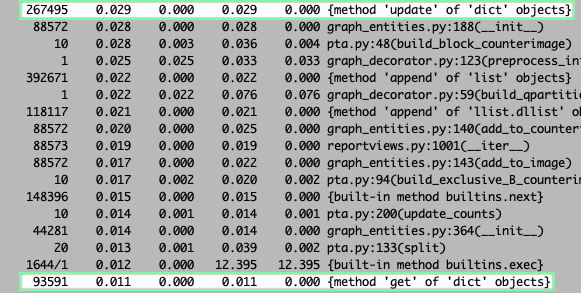
\includegraphics[width=0.7\textwidth]{./sezione3/future/resources/profiler.png}
    \caption{Output fornito da cProfile per una delle funzioni implementate nel pacchetto, sono evidenziate le righe corrispondenti ad interrogazioni o aggiornamenti di un dizionario.}
    \label{fig:cprofile_result}
\end{figure}

Intendiamo continuare lo sviluppo del pacchetto poichè riteniamo che il progetto meriti di essere sviluppato ulteriormente, e non ne abbiamo trovati altri in Python che trattino la bisimulazione in modo approfondito.


\clearpage

\newpage

\renewcommand\refname{Bibliografia}
\bibliographystyle{plain}
\bibliography{bibliography}

\end{document}
